\documentclass[a4paper,10pt]{article}
\usepackage[spanish]{babel}
\usepackage[utf8]{inputenc}
\usepackage[breaklinks=true]{hyperref}
\usepackage{verbatim}
\usepackage{amsmath}
\usepackage{graphicx}
\usepackage{subfig}
%\usepackage{subfigure}
\RequirePackage{fontawesome}
%opening

\begin{document}

\begin{titlepage}
\centering
{
\includegraphics[width=0.9\textwidth]{fing_uncuyo}\par}
\vspace{1cm}
{\bfseries\LARGE Universidad Nacional de Cuyo \par}
\vspace{1cm}
{\scshape\Large Facultad de Ingeniería \par}
\vspace{3cm}
{\scshape\Huge Predicción de Precios de Criptomonedas con ARIMA y Prophet \par}
\vspace{3cm}
{\itshape\Large Proyecto Final\\Inteligencia Artificial I \par}
\vfill
{\Large MOLINA, Mauro \par}
{\Large FLORES, Daniel Emiliano \par}
\vfill
{\Large Marzo 2022 \par}
\end{titlepage}

\newpage

\tableofcontents

\newpage

\section{Introducción}

\subsection{Criptomonedas}

 Una criptomoneda es un activo digital que emplea un cifrado para garantizar integridad, autenticidad y confidencialidad de las transacciones, es decir, funcionan como moneda de cambio y solucionan los problemas que las monedas de cambio tradicionales presentan.

 El dinero reemplazó a la economía de trueque, donde las transacciones se rigen bajo la premisa ``¿cuánto de mi producto vale el tuyo?''. Para sustituir esta modalidad, el valor de un producto o servicio se mide en función del dinero.

La moneda se puede abstraer como cualquier objeto (real o no) que resuelva sea capaz de cumplir esta característica. Formalmente, debe cumplir los siguientes aspectos:

\begin{itemize}
 \item Debe servir como moneda de cambio, es decir, quien aporta el capital recibe un bien o servicio a cambio.
 \item Debe servir de referencia de valor, es decir, poder determinar, a través de dicha moneda, cuánto vale un bien o servicio.
 \item Debe servir como reserva de valor, es decir, que su valor no se vea moficado con el paso del tiempo.
\end{itemize}

Estos parámetros son determinados por la sociedad, según el uso y confianza que le tengan a la moneda.

Las criptomonedas no son diferentes a las monedas corrientes, con algunas salvedades:

\begin{itemize}
 \item No hay un ente central del que dependamos (como el banco) que regule las transacciones.

 \item Mantiene total privacidad, ya que toda la información está encriptada y nadie sabe la información del dueño del dinero.

 \item Evita problemas de "devaluación" de la moneda, ya que no depende de factores socio-económicos (como la emisión monetaria)
\end{itemize}

Este sistema funciona bajo el modelo Peer-To-Peer (P2P), donde cada usuario funciona como cliente o servidor de otro, según corresponda. Es decir, si queremos saber cuanto dinero tiene una persona, debemos mantener un registro global, que incluye a todas las transacciones que han ocurrido desde el origen de una determina criptomoneda. Este registro debe ser público, para que cualquier persona pueda consultarlo en cualquier momento.

Pero si existe este registro ¿cómo puede existir la privacidad?

La privacidad se sigue respetando, ya que realmente no se sabe a quien pertenece el dinero que figura en dichas transacciones. Esta cadena de transacciones se conoce como \textbf{BlockChain} (cadena de bloques). La idea aquí es formar una LinkedList, donde cada bloque apunta al anterior.
Las personas encargadas de añadir los bloques al registro de transacciones se conocen como \textbf{mineros}. Una vez que se añade el bloque a la cadena, se avisa al resto de los mineros que añadan dicho en su registro.

Nótese que un bloque puede contener muchas transacciones.

\subsubsection{Precios}

 El precio se determina por la oferta y la demanda. Cuando se incrementa la demanda, el precio sube, y cuando cae la demanda, el precio baja. Hay un número limitado de criptomonedas en circulación y las nuevas son creadas a una velocidad predecible y decreciente, esto significa que la demanda debe seguir este nivel de inflación para mantener un precio estable. Este es el caso del Bitcoin.

 Sin embargo, en la actualidad es posible crear tokens con emisión ilimitada, a disposición de reglas establecidas (por ejemplo, ADA) o el sistema de recompensas (CAKE).

 Al concluir el desarrollo teórico del presente informe, se evaluarán los resultados sobre las criptomonedas Bitcoin [BTC], Ether [ETH] y Ada [ADA].

\subsection{Series Temporales}

Una serie de tiempo es una forma estructurada u ordenada de presentar los datos, en donde un parámetro temporal regular o irregular (fecha, hora, semana, día, mes, año, etc.) lleva asociado un valor.

Se usan para estudiar la relación causa-consecuencia entre diversas variables que cambian con el tiempo. Desde el punto de vista probabilístico, una serie temporal es una sucesión de variables aleatorias indexadas según parámetro creciente con el tiempo, que conforman un conjunto ordenado de datos y coexisten de forma dependiente entre ellas.

Con la ayuda del machine learning, puede servir para detectar patrones implicitos en el comportamiento de los fenómenos con el solo hecho de ordenarlos según un parámetro temporal.

Por ejemplo: Un caso trivial podría ser el de realizar una serie temporal con las ventas del año de una heladería. El resultado en este caso es trivial. Las ventas alcanzan un maximo relativo en verano y un mínimo relativo en invierno.

El instrumento de análisis que se suele utilizar es
un modelo que permita reproducir el comportamiento de la variable de interés. Estos pueden ser:

\begin{itemize}
 \item Univariantes: la serie temporal es analizada únicamente en función de su propio pasado;

 \item Multivariantes: son analizadas varias series temporales, en consecuencia a la suposición de dependencia o relación entre ellas.
\end{itemize}

Describimos matemáticamente una serie temporal univariante como un conjunto de observaciones, de tamaño $T$, sobre una variable $Y$:

\begin{equation}
 Y_t, \quad t = 1,2,...,T
\end{equation}



El pronóstico de la serie temporal implica extender los valores históricos hacia el futuro, tales como el periodo y el horizonte (cantidad de periodos proyectados). Si es un modelo univariante, se pronostica únicamente en términos de valores pasados $Y_t$, lo que comunmente llamamos extrapolación.

Si una serie temporal es extrapolable exactamente, decimos que ésta es determinista. Sin embargo, la gran parte de ellas no lo son y están condicionadas a una distribución de probabilidad dependiente de sus valores pasados.

Los modelos utilizados para caracterizar una serie temporal responden siempre a una misma fórmula:

\begin{equation}\label{eqn:sistinnov}
 Y_t = S_t + a_t
\end{equation}

Donde $S_t$ indica el comportamiento regular de la variable -conocida como parte sistémica- y $a_t$ es el comportamiento aleatorio -tambien denominada \textit{innovación}-.

En modelos de series univariantes, $S_t$ se determina únicamente en función del pasado de la serie:

\begin{equation}
 S_t = f(Y_t, Y_{t-1}, Y_{t-2},...)
\end{equation}



\subsubsection{Análisis de las Series Temporales}

Las series temporales pueden ser descritas en función de sus componentes. En ciertos modelos, son resultado de cuatro componentes que actúan en conjunto:

\begin{itemize}

 \item \textbf{Tendencia secular o regular.} Indica el crecimiento, decrecimiento o estacionalidad general y persistente del fenómeno observado, es la componente que refleja la evolución a largo plazo. La denotaremos como $B_t$.

 \item \textbf{Variación estacional o variación cíclica regular.} Está relacionada con el movimiento periódico de corto plazo. Se trata de una componente causal debida a la influencia de ciertos fenómenos que se repiten de manera periódica en un periodo de tiempo. Por ejemplo, si el periodo es un año, las estaciones son una variacion cíclica regular, si el periodo es una semana, los fines de semana son la variación estacional, si el periodo es un día, las horas son la variación estacional. Recopila las oscilaciones que se producen en esos períodos temporales regulares. La denotaremos como $E_t$.

\item \textbf{Variación cíclica.} Recoge las oscilaciones periódicas de amplitud superior a un año. Movimientos normalmente irregulares alrededor de la tendencia, en las que, a diferencia de las variaciones estacionales, tiene un período y amplitud variables. En otras palabras, son variaciones estacionales de largo plazo y de eventos irregulares. Esta componente puede no existir, ya que la serie temporal puede no ser cíclica en ningún momento. La denotaremos como $C_t$.

 \item \textbf{Variación aleatoria o ruido.} Incluye todos aquellos factores que no muestran ninguna regularidad, debidos a fenómenos de carácter ocasional. Por ejemplo: Tormentas en relación con las cosechas de alguna verdura. La denotaremos como $R_t$.

\end{itemize}

Estas componentes generan los siguientes tipos de series:

\begin{itemize}
 \item \textbf{Aditivas.} Sumando sus componentes: $X_t = B_t + E_t + C_t + R_t$

 \item \textbf{Multiplicativas.} Multiplicando sus componentes: $X_t = B_t * E_t * C_t * R_t$

 \item \textbf{Mixtas.} Sumando y multiplicando sus componentes, por lo que existen varias alternativas. Por ejemplo: $X_t = B_t + E_t * C_t * R_t$
\end{itemize}

Sin embargo, la clasificación arriba descrita no es utilizada para modelos ARIMA. En estos, se trata de obtener la representación de la serie en términos de la interrelación temporal entre sus elementos.

\subsubsection{Coeficiente de autocorrelación}

Uno de los instrumentos utilizados es el coeficiente de correlación $\rho_{xy}$ entre dos variables $x_t$ y $y_t$. Este coeficiente mide el grado de asociación lineal entre ellas:

\begin{equation}
 \rho_{xy} = \frac{cov(x,y)}{\sqrt{V(x)V(y)}}
\end{equation}

donde, por definición, $\rho_{xy} \in [-1,1]$.

De este coeficiente de correlación poblacional podemos estimar el coeficiente de correlación muestral:

\begin{equation}
 r_{xy} = \frac{\sum_{t=1}^{T} (x_t - \bar{x}) (y_t - \bar{y})}
 {\sqrt{\sum_{t=1}^{T} (x_t - \bar{x})^2 \sum_{t=1}^{T} (y_t - \bar{y})^2 } }
\end{equation}

Si tenemos $T$ observaciones $Y_1,..., Y_T$, podemos crear ($T-1$) pares de observaciones ($Y_1,Y_2),...,(Y_{T-1},Y_T)$. Es decir, consideramos $Y_1,...,Y_{T-1}$ como una variable y $Y2,...,Y_T$ como otra para definir la correlación entre ambas variables $Y_t,Y_{t+1}$:

\begin{equation}
 r_{Y_t Y_{t+1}} = \frac{\sum_{t=1}^{T-1} (Y_t - \bar{Y}_{(1)}) (Y_{t+1} - \bar{Y}_{(2)})}
 {\sqrt{\sum_{t=1}^{T-1} (Y_t - \bar{Y}_{(1)})^2 \sum_{t=1}^{T-1} (Y_{t+1} - \bar{Y}_{(2)})^2 } }
\end{equation}

Donde $\bar{Y}_{(1)}$ y $\bar{Y}_{(2)}$ es la media muestral de las primeras $T-1$ observaciones y la media muestral de las últimas $T-1$ observaciones, respectivamente.

La expresión anterior es aproximadamente:

\begin{equation}
 r_{Y_t Y_{t+1}} \approx r_1 = \frac{\sum_{t=1}^{T-1} (Y_t - \bar{Y}) (Y_{t+1} - \bar{Y})}
 {\sum_{t=1}^{T} (Y_t - \bar{Y})^2 }
\end{equation}

El subíndice indica el intervalo de correlación lineal de las observaciones analizadas. En el caso anterior descrito, $r_1$ analiza observaciones sucesivas y se denomina \textit{coeficiente de autocorrelación de primer orden}.

Por tanto, el coeficiente de autocorrelación de orden $k$ viene dado por:

\begin{equation}
 r_k = \frac{\sum_{t=1}^{T-k} (Y_t - \bar{Y}) (Y_{t+k} - \bar{Y})}
 {\sum_{t=1}^{T} (Y_t - \bar{Y})^2 }
\end{equation}

Para interpretar el conjunto de los coeficientes de autocorrelación de una serie temporal se utiliza un \textit{correlograma}, que es un gráfico que agrupa los $k$ coeficientes de autocorrelación.

Estos suelen comenzar en $k=1$ puesto que un $k=0$ en la Ecuación (8) siempre es $1$.

\begin{enumerate}
 \item Si una serie es puramente aleatoria, $r_k \approx 0$ para cualquier $k \neq 0$ siendo $T$ suficientemente grande.

 \item Series sin tendencia oscilantes en torno a una media constante:

 \begin{enumerate}
  \item Si contiene observaciones por encima de la media seguidas de una o más observaciones por encima de la media (lo mismo para observaciones por debajo de la media), entonces $r_k$ decrece tendiendo a cero rápidamente a medida que aumenta $k$.

  \item Si contiene observaciones alternantes por encima y debajo de la media, el correlograma presenta valores decrecientes que alternan su signo.
 \end{enumerate}

  \item Si la serie contiene una tendencia, los valores de $r_k$ no decrecerán a cero rápidamente. Esto se debe a que un valor observado tiene sucesivos valores que estarán por encima (o debajo) de la media. Este tipo de comportamiento nos da poca información.

  \item Si una serie presenta algún tipo de ciclo, el correlograma también presentará una oscilación a la misma frecuencia. En las series con un comportamiento cı́clico permanente, el correlograma da de nuevo poca información porque lo domina el comportamiento cı́clico presente en los datos.
\end{enumerate}





\section{Procesos Estocásticos}

Un proceso estocástico es una familia de variables aleatorias relacionadas entre sí y que siguen una ley de distribución conjunta. Lo denotaremos por:

\begin{center}
 $...,Y_{t-2},Y_{t-1},Y_t,Y_{t+1},Y_{t+2},...$ o $Y_t$
\end{center}

A simple vista podemos entender que fijar $t=t_0$ nos dá una variable aleatoria de la secuencia \textit{presumiblemente ordenada}\footnote{El orden en la sucesión de observaciones es único en una serie temporal. Alterarlo implicaría modificar las características de la serie.}. Además, llamaremos \textit{realización} del proceso a la asignación de un valor a cada una de las variables aleatorias del mismo.

En virtud de lo anterior, una serie temporal $Y_t, Y_{t+1},Y_{t+2},...$ se puede interpretar como una realización muestral de un proceso estocástico para un número finito de periodos $t=1,2,...,T$.

\subsection{Características}

\textbf{Función de distribución.} Incluye todas las funciones de distribución para cualquier subconjunto finito de variables aleatorias del proceso:

\begin{center}
$F[Y_{t_i}, Y_{t_{i+1}},...,Y_{t_n}]$ siendo $n$ finito.
\end{center}

\textbf{Momentos del proceso estocástico.} El primer momento de un proceso estocástico es el conjunto de las medias de todas las variables aleatorias del proceso:

\begin{equation}
E(Y_t) = \mu_t < \infty, \quad t = 0, \pm 1, \pm 2, ...
\end{equation}

El segundo momento viene dado por el conjunto de las varianzas de todas las variables aleatorias del proceso y por las covarianzas entre todo par de variables aleatorias:

\begin{equation}
\begin{split}
V(Y_t) & = E[Y_t - \mu_t]^2 = \sigma_t^2 < \infty, \quad t=0, \pm 1, \pm 2, ... \\
cov(Y_t,Y_s) & = E[Y_t - \mu_t][Y_s - \mu_s] = \gamma_{t,s} \quad \forall t,s \quad (t \neq s)
\end{split}
\end{equation}

\subsection{Procesos estocásticos estacionarios}

Para hacer análisis y predicciones consistentes a una serie de tiempo, es necesario que la estructura probabilística que subyace en el proceso estocástico sea estable en el tiempo. Es decir, las regularidades del comportamiento pasado deben ser capaces de proyectarse a futuro. Estas características de un proceso estocástico se las conoce como \textit{estacionariedad}.

\textbf{Estacionariedad estricta.} Un proceso estocástico es estrictamente estacionario si y solo si

\begin{equation}
F[Y_{t_i}, Y_{t_{i+1}},...,Y_{t_n}] = F[Y_{t_i+k}, Y_{t_{i+1}+k},...,Y_{t_n+k}]
\end{equation}

en otras palabras, si la función de distribución de cualquier conjunto finito de variables aleatorias del proceso no se altera si se desplaza $k$ periodos en el tiempo.

\textbf{Estacionariedad en covarianza.} Un proceso estocástico es estacionario en covarianza si y solo si:

\begin{enumerate}
 \item Es estacionario en media, es decir, todas las variables aleatorias tienen la misma media y es finita:
 \begin{equation}
  E(Y_t) = \mu < \infty, \quad \forall t
 \end{equation}

 \item Todas las variables aleatorias tienen la misma varianza y es finita:
 \begin{equation}\label{eqn:varianza}
  V(Y_t) = E[Y_t - \mu]^2 = \sigma_Y^2 < \infty, \quad \forall t
 \end{equation}

 \item La covarianza lineal entre dos variables aleatorias del proceso que disten $k$ periodos de tiempo es la misma que existe entre cualesquiera otras dos variables que estén separadas también $k$ periodos. También conocemos esta propiedad como \textit{autocovarianza}:
 \begin{equation}\label{eqn:covarianza}
  cov(Y_t,Y_s) = E[Y_t - \mu][Y_s - \mu] = \gamma_{t,s} = \gamma_{|t-s|} = \gamma_k \quad \forall k
 \end{equation}

\end{enumerate}

Finalmente, decimos que un proceso estocástico estacionario en covarianza está caracterizado si se conoce:

\begin{center}
$\mu, \quad V(Y_t), \quad \gamma_k, \quad k=0$,\pm 1, \pm 2,...
\end{center}

Si bien las series económicas no presentan comportamientos estacionarios, particularmente las series temporales que reflejan el precio de una criptomoneda, se procederá a proponer modelos que para procesos estacionarios. A partir de estos se puede modelar para un proceso no estacionario.

\subsection{Formalización de funciones}

\textbf{Función de autocovarianzas.} Es una función de $k$ (número
de periodos de separación entre las variables) que recoge el conjunto de las autocovarianzas del proceso estocástico estacionario:

\begin{center}
$\gamma_k$, $k=0,1,2,...$
\end{center}

Es una función simétrica:

\begin{center}
$\gamma_k = \gamma_{-k}$
\end{center}

y, además, incluye la varianza del proceso para $k=0$:

\begin{center}
$\gamma_0 = V(Y_t)$.
\end{center}

\textbf{Función de autocorrelación.} Al igual que la anterior, recoge toda la información de la estructura dinámica lineal del proceso estocástico con la diferencia de que es independiente de las unidades de la variable.

El coeficiente de autocorrelación de orden $k$ de un proceso estocástico estacionario mide el grado de asociación lineal existente entre dos variables aleatorias del proceso separadas por $k$ periodos:

\begin{equation}
\rho_k = \frac{cov(Y_t, Y_{t+k})}{\sqrt{V(Y_t)*V(Y_{t+k)}}} = \frac{\gamma_k}{\sqrt{\gamma_0 * \gamma_0}} = \frac{\gamma_k}{\gamma_0}
\end{equation}

donde

\begin{center}
$|\rho_k| \leq 1$, $\forall k$
\end{center}

La función de autocorrelación de un proceso estocástico estacionario es una función de $k$ que
recoge el conjunto de los coeficientes de autocorrelación del proceso y se denota por $\rho_k$. La función de autocorrelación se suele representar gráficamente por medio de un correlograma.

El coeficiente de autocorrelación de orden 0 es, por definición, 1. Genera una función simétrica, por lo que un correlograma solo representa valores positivos de $k$. Esta función, además, tiende a cero rápidamente a medida que $k$ tiende a infinito. Ésta última afirmación es correcta cuando tenemos un proceso estocástico estacionario, condición que se buscará y se hará énfasis en el análisis de resultados.

De estas premisas, al observar un correlograma podemos concluir que su correspondiente serie no es estacionaria si la función no decrece rápidamente.

\subsubsection{Estacionaridad y estimación de momentos}

Si la serie temporal $(Y_1,Y_2,...,Y_T)$ no fuera estacionaria, ya no tendríamos una única media, ni una única varianza y las autocorrelaciones serían demasiadas. La estacionaridad es, desde luego, una restricción necesaria para estimar los momentos de un proceso estocástico.

\subsection{Ruido blanco}

El proceso estocástico ruido blanco, denotado $w_t$, lo definimos como:

\begin{equation*}
\begin{split}
E(w_t) &= 0, \forall t \\
V(w_t) &= \sigma^2, \forall t \\
Cov(w_t,w_s) &= 0, \forall t \neq s \\
\end{split}
\end{equation*}

Un proceso ruido blanco $w_t ~ RB(0,\sigma^2)$ es estacionario si la varianza $\sigma^2$ es finita, con función de autocovarianzas:

\begin{equation*}
\gamma_k= \left\{ \begin{array}{lcc}
             \sigma^2, \quad k=0 \\
             0, \quad k > 0
             \end{array}
   \right.
\end{equation*}

y función de autocorrelación:

\begin{equation*}
\rho_k= \left\{ \begin{array}{lcc}
             1, \quad k=0 \\
             0, \quad k > 0
             \end{array}
   \right.
\end{equation*}

\section{Modelos estacionarios}

La estructura de dependencia temporal de una serie está recogida en la función de autocovarianzas y/o en la función de autocorrelación. Mediante un modelo ARMA, se tratará de reproducir el comportamiento general y posteriormente predecir con la ayuda del mismo.

\subsection{Modelo Lineal General}

Anteriormente descompusimos una serie temporal univariante en dos componentes (\ref{eqn:sistinnov}). Ahora, nuestra parte sistémica contiene la información para construir el modelo mientras que la innovación contendrá valores sin dependencia entre sí, tanto en valores pasados como con su parte sistémica. La innovación, como se habrá podido intuir, es el ruido blanco.

Así, un modelo teórico capaz de describir un comportamiento de una serie temporal con media cero sería:

\begin{equation}
Y_t = f(Y_{t-1},Y_{t-2},...) + w_t, \quad t=1,2,...
\end{equation}

El proceso estocástico puede responder a un proceso de Gauss, por lo que $Y_t$ puede expresarse como una combinación lineal de sus valores pasados infinitos más una innovación:

\begin{equation}\label{eqn:ar}
Y_t = \pi_1 Y_{t-1} + \pi_2 Y_{t-2} + ... + w_t \quad t=1,2,...
\end{equation}

donde $Y_t$ es un proceso estacionario y $\pi_i$ son constantes con $\phi_t \neq 0$.

Para que esto suceda, es preciso que el proceso sea \textit{no anticipante}: cualquier valor $Y_i$ no debe depender de valores futuros. En adición, el proceso debe ser \textit{invertible}, es decir que el presente dependa de forma convergente con su propio pasado. A medida que nos alejemos en el tiempo, la influencia de $Y_k$ debe disminuir. Esta restricción viene dada por:

\begin{equation*}
 \sum_{i=1}^\infty \pi_i^2 < \infty
\end{equation*}


\textbf{Operador de retardos.} Lo definimos como:

\begin{equation}
BY_t = Y_{t-1}
\end{equation}

particularmente:

\begin{equation*}
B^2Y_t = B(BY_t) = BY_{t-1} = Y_{t-2}
\end{equation*}

y generalmente:

\begin{equation}
B^kY_t = Y_{t-k}
\end{equation}

Reescribimos (\ref{eqn:ar}) en función del operador de retardos:

\begin{center}
$Y_t = (\pi_1B + \pi_2B^2 + ...) Y_t + w_t$

$(1-\pi_1B - \pi_2 B^2 - ...) Y_t = w_t$
\end{center}

Si $(1-\pi_1B - \pi_2 B^2 - ...) = \pi_\infty(B)$:

\begin{equation}\label{eqn:infinit}
\pi_\infty(B)Y_t = w_t
\end{equation}

Teniendo presente que $\pi_\infty(B)$ es un polinomio de orden infinito, es necesario aproximarlo a uno de orden finito -los modelos a desarrollar deberán representar procesos estocásticos acotados en el tiempo:

\begin{equation}\label{eqn:finit}
\pi_\infty(B) \approx \frac{\phi_p(B)}{\theta_q(B)}
\end{equation}

donde:

\begin{equation}
\begin{split}
\phi_p(B) &= 1 - \phi_1B - \phi_2B^2 - ... - \phi_pB^p \\
\theta_p(B) &= 1 - \theta_1B - \theta_2B^2 - ... - \theta_qB^q
\end{split}
\end{equation}

Sustituyendo (\ref{eqn:finit}) en (\ref{eqn:infinit}):

\begin{equation}
\phi_p(B) Y_t = \theta_q (B) w_t
\end{equation}

Por lo tanto, este modelo lineal general admite tres representaciones:

\begin{itemize}
 \item \textit{Puramente regresiva, AR($\infty$):} el valor presente de la variable se representa en función de su propio pasado más una innovación contemporánea.

 \item \textit{Puramente de medias móviles, MA($\infty$):} el valor presente de la variable se representa en función de todas las innovaciones pasadas y presente.

 \item \textit{Finita:}

 \begin{equation}\label{eqn:completa}
 \begin{split}
 &(1-\phi_1B - \phi_2B^2 - ... - \phi_pB^p) Y_t = (1-\theta_1B - \theta_2B^2 - ... - \theta_qB^q) w_t \\
 &Y_t = \phi_1Y_{t-1} + \phi_2Y_{t-2} + ... + \phi_pY_{t-p} + w_t -\theta_1w_{t-1} - \theta_2w_{t-2} - ... - \theta_qw_{t-q}
 \end{split}
 \end{equation}

 Este modelo se denomina \textit{Autorregresivo de Medias Móviles} de orden $(p,q)$. En él, el valor de $Y_t$ depende del pasado de $Y$ hasta el momento $t-p$ de la innovación contemporánea y su pasado hasta el momento $t-q$.
\end{itemize}

\subsection{Procesos Autoregresivos de Medias Móviles}

Como hemos señalado anteriormente, la ecuación \ref{eqn:completa} es una aproximación finita al modelo lineal general tanto en su forma $AR(\infty)$ como $MA(\infty)$.

De hecho, si es estacionario su representación $MA(\infty)$ es

\begin{equation}
Y_t = \frac{\theta_q(B)}{\phi_p(B)} w_t \quad \to \quad Y_t = \psi_\infty(B) w_t \quad \to \quad Y_t = w_t + \psi_1 w_{t-1} + \psi_2 w_{t-2} + ...
\end{equation}

y si es invertible, su representación $AR(\infty)$ es

\begin{equation}
\frac{\phi_p(B)}{\theta_q(B)} Y_t = w_t \quad \to \quad \pi_\infty(B) Y_t = w_t \quad \to \quad Y_t = w_t + \pi_1 Y_{t-1} + \pi_2 Y_{t-2} + ...
\end{equation}

\textbf{Teorema de estacionariedad.} Un proceso autoregresivo de medias móviles finito $ARMA(p,q)$ es estacionario sí y solo sí el módulo de las raíces del polinomio autorregresivo $\phi(B)$ está fuera del círculo unidad.

Las condiciones de estacionariedad del modelo $ARMA(p,q)$ vienen impuestas por la parte autorregresiva, dado que la parte de medias móviles finita siempre es estacionaria.

Para comprobar si el modelo $ARMA(p,q)$ es no anticipante e invertible , se estudia su representación autorregresiva general.

\textbf{Teorema de invertibilidad.} Un proceso autorregresivo de medias móviles finito $ARMA(p,q)$ es invertible sí y solo sí el módulo de las raíces del polinomio de medias móviles $\theta_p(B)$ está fuera del círculo unidad.

Las condiciones de invertibilidad del modelo $ARMA(p,q)$ vienen impuestas por la parte de medias móviles, dado que la parte autorregresiva finita siempre es invertible porque está directamente escrita en forma autorregresiva

El modelo $ARMA(p,q)$ tiene media cero, varianza constante y finita y una función de autocovarianzas infinita. La función de autocorrelación es infinita decreciendo rápidamente hacia cero pero sin truncarse.

\subsubsection{$ARMA(1,1)$}

En este modelo, $Y_t$ se determina en función de su pasado hasta el primer retardo, la innovación contemporánea y el pasado de la innovación hasta el retardo 1:

\begin{equation}
Y_t = \phi Y_{t-1} + w_t - \theta w_{t-1} \qquad w_t ~ RB (0,\sigma^2) \qquad t=1,2,...
\end{equation}


La memoria de este proceso es larga debido a que presenta la estructura autorregresiva. Es decir, una perturbación $w_t$ ingresa al sistema afectando a $Y_t$ y, a través de él, al futuro. Sin embargo, por su estructura de medias móviles, la perturbación $w_t$ afecta directamente a $Y_t$ $Y_{t-1}$.

\begin{equation*}
\begin{split}
& ... \quad \to \quad Y_{t-2} \quad \to \quad Y_{t-1} \quad \to \quad Y_{t} \quad \to \quad Y_{t+1} \quad \to \quad Y_{t+2} \to ... \\
& \quad \quad \quad \quad \quad \uparrow \quad \quad \nearrow \quad \quad \uparrow \quad \quad \nearrow \quad \;\; \uparrow \quad \;\; \nearrow \quad \quad \uparrow \quad \quad \nearrow \quad \quad \uparrow \quad \quad \nearrow \\
& \quad ...\quad \quad \;\; w_{t-2} \qquad \quad \; \; w_{t-1} \qquad \quad \:\: w_{t} \qquad \quad \; w_{t+1} \qquad \quad \;\; w_{t+2}
\end{split}
\end{equation*}

Por el teorema de estacionariedad, es necesario y suficiente comprobar que las raíces del polinomio autorregresivo estén fuera del círculo unidad:

\begin{equation*}
\phi_1(B) = 1 - \phi B = 0 \quad \to \quad B = \frac{1}{\phi} \quad \to \quad |B| = |\frac{1}{\phi}| \quad \to \quad |\phi| < 1
\end{equation*}

Por el teorema de invertibilidad, es necesario y suficiente comprobar que las raíces del polinomio de medias móviles estén fuera del círculo unidad:

\begin{equation*}
\theta_1(B) = 1 - \theta B = 0 \quad \to \quad B = \frac{1}{\theta} \quad \to \quad |B| = |\frac{1}{\theta}| \quad \to \quad |\theta| < 1
\end{equation*}

La media de este proceso es:

\begin{equation*}
\begin{split}
E(Y_t) = E(\phi Y_{t-1} + w_t - \theta w_{t-1}) &= \phi E(Y_t) \\
\to \quad (1-\phi)E(Y_t) &= 0 \\
\to \quad E(Y_t) &= 0
\end{split}
\end{equation*}

Para determinar la función de covarianzas, tenemos en cuenta que:

\begin{equation*}
E(Y_{t-1}w_{t-1}) = E[(\phi Y_{t-2} + w_{t-1} - \theta w_{t-2})w_{t-1}] = E(w_{t-1})^2 = \sigma^2
\end{equation*}


En tanto, dicha función es:

\begin{equation*}
\begin{split}
\gamma_0 &= E(Y_t - E(Y_t))^2 = E(Y_t)^2 = E(\phi Y_{t-1} + w_t - \theta w_{t-1})^2 \\
&= \phi ^2 E(Y_{t-1})^2 + E(w_t)^2 + \theta^2 E(w_{t-1})^2 + 2\phi E(Y_{t-1}w_t) - 2\phi \theta E(Y_{t-1}w_{t-1}) - 2\theta E(w_t w_{t-1}) \\
&= \phi^2 \gamma_0 + \sigma^2 + \theta^2 \sigma^2 - 2\phi \theta \sigma^2 \\
&= \phi^2 \gamma_0 + (1+\theta^2 - 2\phi\theta) \sigma^2 \\
\to \quad \gamma_0 &= \frac{(1+\theta^2 -2\phi \theta)\sigma^2}{1-\phi^2}\\
\\ %gamma 1 ###################################################
\gamma_1 &= E(Y_t - E(Y_t))(Y_{t-1} - E(Y_{t-1})) = E(Y_tY_{t-1}) \\
&= E[(\phi Y_{t-1} + w_t - \theta w_{t-1})Y_{t-1}] \\
&= \phi E(Y_{t-1})^2 +E(Y_{t-1}w_t) - \theta E(Y_{t-1} w_{t-1}) \\
&= \phi \gamma_0 - \theta \sigma^2 \\
\\ %gamma 2 ##################################################
\gamma_2 &= E(Y_t - E(Y_t))(Y_{t-2} - E(Y_{t-2})) = E(Y_tY_{t-2}) \\
&= E[(\phi Y_{t-1} + w_t - \theta w_{t-1})Y_{t-2}] \\
&= \phi E(Y_{t-1}Y_{t-2}) +E(Y_{t-2}w_t) - \theta E(Y_{t-2} w_{t-1}) \\
&= \phi \gamma_1 \\
\end{split}
\end{equation*}

Es decir que la función de autocovarianzas para un $ARMA(1,1)$ es:

\begin{equation*}
\gamma_k= \left\{ \begin{array}{lcc}
             \frac{(1+\theta^2 -2\phi\theta) \sigma^2}{1-\phi^2} , \quad k=0 \\
             \phi \gamma_0 - \theta \sigma^2 , \quad k=1 \\
             \phi \gamma_{k-1} , \quad k>1
             \end{array}
   \right.
\end{equation*}


La función $\gamma_k$ nos brinda un formalismo a lo expresado previamente. La autocovarianza de orden 0 cuenta con términos provenientes de la parte autorregresiva y de medias móviles. De forma similar, en la autocovarianza de orden 1 tenemos términos de $AR(1)$ $MA(1)$. Finalmente, órdenes superiores dependen exclusivamente de la autorregresión.

La función de autocorrelación de un $ARMA(1,1)$ es:

\begin{equation*}
\rho_k= \left\{ \begin{array}{lcc}
             \phi - \frac{\theta \sigma^2}{\gamma_0} , \quad k=1 \\
             \phi \rho_{k-1}
             \end{array}
   \right.
\end{equation*}

La FAC presenta la misma estructura que la función de autocovarianzas, es decir, es una función
infinita cuyo primer coeficiente, $\rho_1$ , depende de los parámetros autorregresivos y de medias
móviles, pero a partir del retardo 2, decrece exponencialmente, siguiendo la estructura dada
por la parte autorregresiva de orden 1.

\subsubsection{$ARMA(p,q)$}

Los resultados obtenidos para $ARMA(1,1)$ son generalizables para este modelo. Observemos: para los primeros $q$ coeficientes $\rho_1, ..., \rho_q$ dependerán de los parámetros autorregresivos y de medias móviles, mientras que los siguientes no dependerán del parámetro de medias móviles. En consecuencia, la función de autocorrelación decrecerá rápidamente a cero.

Es posible modificar $ARMA(p,q)$ de tal forma que su media no sea nula añadiendo una constante al proceso estacionario:

\begin{equation}
Y_t = \delta + \phi_1Y_{t-1} + \phi_2Y_{t-2} + ... + \phi_pY_{t-p} + w_t -\theta_1w_{t-1} - \theta_2w_{t-2} - ... - \theta_qw_{t-q} \qquad w_t ~ RB(0,\sigma^2)
\end{equation}

La única diferencia respecto al modelo sin la constante $\delta$ es que su media no es cero:

\begin{equation*}
\begin{split}
E(Y_t) &= E(\delta + \phi_1 Y_{t-1} +...+ \phi_p Y_{t-p} + w_t + \theta_1 w_{t-1} + ... + \theta_q w_{t-q})\\
& = \delta + \phi_1 E(Y_t) + ... + \phi_p E(Y_{t})\\
\to \quad \delta &= (1-\phi_1-...-\phi_p) E(Y_t) \\
E(Y_t) & = \frac{\delta}{(1-\phi_1-...-\phi_p)}
\end{split}
\end{equation*}

\begin{comment}
# Modelo ARMA

El nombre ARMA es la abreviatura de Modelos Autorregresivos de Media Móvil. Proviene de la fusión de dos modelos más simples:
  1) **_El autorregresivo o AR:_** Es una representación de un proceso aleatorio, en el que la variable de interés depende de sus observaciones pasadas. La forma genérica de representar un AR sería la siguiente.
     - _C_: Es la posición inicial, o el último valor leido de la serie.
     - _θ_: Algún factor multiplicativo.
     - _Y_<sub>t-1</sub>: El valor leído anteriormente
     - _ε_<sub>t</sub>: Termino de error
      <p align="center">
          <img src=https://economipedia.com/wp-content/uploads/Modelo-AR-1-formula.png />
      </p>

     _NOTA: Nótese que una regresión puede estar compuesto por un conjunto de valores pasados._


  2) **_El promedio móvil o MA:_** Es un promedio de valores que se va modificando a lo largo del tiempo. La media móvil es un indicador de tendencia que nunca se anticipa a la tendencia de las cotizaciones, es decir, simplemente sigue a la curva de cotizaciones confirmando la tendencia en cada momento.
  <br><br>Existen varios modelos:
      - **Media Móvil Simple:** Recoge el dato que se genera en la última sesión, y a su vez, descarta el dato más antiguo de la serie temporal. La duda que existe es ¿Cuántos términos considerar? <br>

        <p align="center">
          <img src=https://user-images.githubusercontent.com/63267942/149024008-9cab5989-be52-4655-a84f-e013cec55b21.png />
        </p>

        - Si elegimos un **_n_** bajo, nuestra predicción tendrá una alta capacidad para responder rápidamente ante fluctuaciones, ya que la pendiente no se ve influenciada por muchos datos. En contraparte, se vé muy influenciada por los factores aleatorios por la misma razón.<br><br>
        - Si elegimos un **_n_** alto, nuestra predicción filtra o anula los factores aleatorios, ya que no influyen mucho en un promedio de datos grandes, pero presenta cierta inflexibilidad para adaptarse a cambios drásticos válidos en el corto plazo.<br>

          _NOTA: Un problema con esta serie es que cambia 2 veces al leer un nuevo dato, primero por leer un dato nuevo, y segundo por sacar un dato viejo_

      - **Media Móvil Ponderada:** Para evitar que los datos viejos afecten significativamente a la predicción de la serie, se utilizan las medias móviles ponderadas, donde a medida que los datos se vuelven viejos, pierden valor. La idea atrás de este método es que como los datos ya son muy antiguos, no son rendundates para los valores actuales. Esto permite que la serie pueda adaptarse con mayor facilidad a los cambios abruptos en el corto plazo, ya que las ultimas lecturas toman mayor redundancia.
         <p align="center">
            <img src=https://user-images.githubusercontent.com/63267942/149025788-1fd63a1a-df6e-49c6-9dc0-0a4b12e575e2.png />
          </p>


      - **Media Móvil Exponencial:** Es un tipo particular de Media Móvil Ponderada que responde a un crecimiento o decrecimiento exponencial, donde los datos antiguos influyen, pero es casi insignificante.

<br>
<br>
<br>
Luego de esta introducción podemos definir matemáticamente a los modelos ARMA. El modelo general de series temporales autorregresivo con media móvil de _p_ términos autorregresivos y _q_ términos de media móvil se expresa como:
<p align="center">
  <img src=https://economipedia.com/wp-content/uploads/Modelo-ARMA.jpg />
</p>
\end{comment}


\section{Modelos no estacionarios}

Lo visto hasta el momento responde a la estacionariedad en covarianza, es decir, media y varianza constantes y finitas junto a autocovarianzas independientes del tiempo. Sin embargo, en series económicas este comportamiento no se replica.

En este caso, quitaremos el supuesto de que tenemos una serie estacionaria en covarianza y mediante algún método transformaremos la serie para estabilizar la covarianza.

\begin{comment}
\subsection{Transformación de la varianza}

Suponemos que la varianza del proceso la podemos expresar mediante una función:

\begin{equation}
V(Y_t) = k f(\mu_t)
\end{equation}

donde $k$ es una constante positiva y $f$ una función conocida. Por otro lado, buscaremos una función $h$ que transforme la serie de tal forma que $h(Y_t)$ tenga varianza constante.

Desarrollaremos la serie de Taylor de primer orden alrededor de $\mu_t$:

\begin{equation}
h(Y_t) \approx h(\mu_t) + (Y_t - \mu_t) h'(\mu_t)
\end{equation}

La varianza de la transformación es aproximable según:

\begin{equation}
V[h(Y_t)] \approx V[h(\mu_t) + (Y_t - \mu_t)h'(\mu_t)] = V(Y_t) [h'(\mu_t)]^2  = k f(\mu_t) [h'(\mu_t)]^2
\end{equation}

Por lo tanto, para que la varianza de la transformación sea constante, debe cumplirse que:

\begin{equation}
h'(\mu_t) = \frac{1}{\sqrt{f(\mu_t)}}
\end{equation}

CONTINUAR
\end{comment}

\subsection{Modelos ARIMA(p,d,q)}

Supongamos el modelo $ARMA(p,q)$:

\begin{equation*}
\Phi_p (B) Y_t = \Theta_q (B) w_t
\end{equation*}

donde el polinomio $AR$ se puede factorizar en función de sus p raíces $B_1,B_2,...B_p$:

\begin{equation*}
\Phi_p (B) = (1-B_1^{-1}B)(1-B_2^{-1}B)...(1-B_p^{-1}B)
\end{equation*}

Si suponemos que $p-1$ raíces son estacionarias (con módulo fuera del círculo unidad) y una de ellas es unitaria, $B_i = 1$, entonces el polinomio $AR$ se puede reescribir como sigue:

\begin{center}
$\Phi_p (B) = (1-B_1^{-1}B)(1-B_2^{-1}B)...(1-B_p^{-1}B) = \varphi_{p-1} (B) (1-(-1)^{-1}B)$

$\Phi_p(B) = \varphi_{p-1} (B) (1-B)$
\end{center}

donde el polinomio $\varphi_{p-1}(B)$ es el producto de los $p-1$ polinomios de orden 1 asociados a las raíces $B_j$ asociadas al círculo unidad. Necesariamente se aclara que es un polinomio estacionario.

Sustituyendo en el modelo $ARMA(p,q)$ obtenemos:

\begin{equation}\label{eqn:arima}
\begin{split}
\varphi_{p-1}(B) (1-B) Y_t &= \Theta_q (B) w_t \\
\varphi_{p-1}(B) \Delta Y_t &= \Theta_q (B) w_t
\end{split}
\end{equation}

Nótese que $\Delta$ es el polinomio que recoge la raíz unitaria.

La ecuación \ref{eqn:arima} representa a un modelo con un comportamiento no estacionario ya que contiene una raíz unitaria. Un proceso $Y_t$ con estas características se le denomina \textit{proceso integrado de orden 1  }

El proceso $AR$ puede contener más de una raíz unitaria, por lo que se puede generalizar el modelo \ref{eqn:arima} como:

\begin{equation}
\varphi_{p-d} (B) \Delta^d Y_t = \Theta_q (B) w_t
\end{equation}

Así mismo, el polinomio $\varphi_{p-d}(B)$ es estacionario porque sus $p-d$ raíces tienen módulo fuera del círculo unidad, y el polinomio $\Delta^d$, de orden $d$, contiene las $d$ raíces unitarias no estacionarias.

Este proceso $Y_t$ con estas características se denomina \textit{proceso integrado de orden d} y se denota por $Y_t \sim I(d)$.

Formalmente, un proceso $Y_t$ es integrado de orden $d$, $Y_t \sim I(d)$, si $Y_t$ no es estacionario, pero su diferencia de orden $d$, $\Delta^d Y_t$, sigue siendo un proceso $ARMA(p-d,q)$ estacionario e invertible.







\section{Prophet}

Este modelo surge por las limitaciones que presentan los modelos SARIMAX, como estacionariedad y valores igualmente espaciados en el tiempo (siendo que esto puede variar mucho en la realidad).

La idea de este algoritmo es plantear a la serie temporal como la suma de 4 componentes:

\begin{equation}
y(t) = g(t) + s(t) + h(t) + \epsilon_t
\end{equation}

donde:

\begin{itemize}
 \item $g(t)$. Describe la tendencia lineal o de crecimiento logístico de largo plazo, creando una función definida por partes en los puntos de cambio (simplificando la predicción).

 Los puntos de cambio son momentos en los datos donde los datos cambian de dirección.

  \item $s(t)$. Función que define la estacionalidad (anual, mensual, semanal, etc.)

  \item $h(t)$. Hechos concretos que pueden alterar los valores de la serie (vacaciones, feriados, paros, etc.), a definirse por el usuario

  \item $\epsilon_t$. Término de error.
\end{itemize}

\subsection{Elementos}

Prophet intenta ajustar las funciones (lineales o no) a los datos dando más o menos importancia a los distintos efectos, es decir, un modelo muy parametrizable:

\begin{enumerate}
 \item \textbf{Tendencia lineal $g(t)$.} Para calcular el termino $g(t)$, Prophet ofrece 2 alternativas.

   \begin{itemize}
    \item Crecimiento Logístico. Estos casos corresponden a situaciones en donde se da una saturación que no permite el crecimiento más allá de un límite determinado. Se aplica una sigmoide pero un poco cambiada.

     - C: Capacidad de Carga. Define la carga máxima que puede llegar a tomar la curva. Nótese que este valor puede no ser fijo y depender de otro parámetro externo C(t).

     - k: Es la tasa de crecimiento. Define qué tan rápido pasará de 0 a la capacidad de carga o viceversa.

     - m: Es un parámetro de compensación. Define el punto de inflexión de la función, es decir, cuando cambia de concavidad.

     \begin{equation}
      g(t) = \frac{C}{1+e^{-k(t-m)}}
     \end{equation}


  \item Modelo Lineal por Partes: Para pronosticar problemas que no muestran un crecimiento saturado, existe una tasa de crecimiento constante por partes.
    $\delta$: tiene los ajustes de tarifas

    k: es la tasa de crecimiento

    m: es el parámetro de compensación, en estos casos, los puntos de quiebre. Los puede definir el usuario o los puede calcular Prophet.

    \begin{equation}
     g(t) = (k+a(t)^T\delta)t + (m+a(t)^T\gamma)
    \end{equation}

  \end{itemize}

 \item \textbf{Ajuste estacional $s(t)$.} Se hace utilizando series de Fourier. Fourier demostró que cualquier función periódica puede formarse a partir de una suma infinita de senos y cosenos.

 \begin{equation}
  s(t) = \sum_{n=1}^N [a_n cos(\frac{2n\pi}{T}t) + b_n sen (\frac{2n\pi}{T}t) ]
 \end{equation}


 \item \textbf{Término h(t).} Queda definido por el usuario, y son aquellos valores que pueden llegar a alterar la serie temporal. Por ejemplo: La llegada del verano altera las ventas de una heladería, los hechos históricos importantes, los fin de semana largos en la venta de vuelos, etc.

 \item \textbf{Error $\epsilon_t$.} Se estima por diferencia.

\end{enumerate}

\subsection{Incertidumbre}

Prophet contempla los casos donde se presenta la incertidumbre en la serie y la clasifica de 3 formas:

\begin{itemize}
 \item Incertidumbre en la tendencia: Prophet puede adaptarse a los cambios de tendencia, pero no anticiparlos. Por ello, asume que en el futuro vendrán cambios de tendencia similares a los de su historia. Esto se calcula con la magnitud, frecuencia y distribución de dichos cambios.

 \item Incertidumbre en la estacionalidad: Por defecto, Prophet asume que no habrá incertidumbre en la estacionalidad, ya que requiere de un muestreo bayesiano completo.

 \item Ruido de observación adicional: Es todo valor, adicional a las incertidumbres, que hacen que nuestra predicción difiera de la realidad.
\end{itemize}



\section{Metodología}


En primer lugar, se obtuvo los datasets para las criptomonedas BTC, ETH y ADA. Se estipuló la extracción para diferentes periodos de tiempo, eligiendo periodos de un día y treinta minutos para cada moneda. Los datos varían entre el 09-11-2017 y 08-03-2022 para el primer caso y 09-02-2022 y 09-03-2022 para el segundo.

Además, se realizó predicciones con periodos de tiempo al azar tomando:

\begin{itemize}
 \item Diez periodos de treinta días, para predecir siete días;
 \item Diez periodos de siete (ARIMA) y ocho (Prophet) días, para predecir siete días.
\end{itemize}

A cada predicción se le extrajeron métricas.

Finalmente, se eligió cuatro periodos de tiempo al azar para los datos del Bitcoin: se comparan sus métricas y la correlación entre la predicción y el valor real, luego entre las predicciones entre sí.


\section{Análisis de Resultados}



\subsection{Métricas}

Un pequeño apartado dedicado a mostrar las métricas de precisión para las series temporales que se utilizarán.

\begin{itemize}

\item Mean Absolute Error [MAE]

Fácil de entender y computar. Recomendada para evaluar la precisión de una sola serie pero para comparar distintas series, con distintas unidades, no es adecuado.

\begin{equation*}
MAE = \frac{1}{n} \sum_{i=1}^n |y_i - \hat{y}_i |
\end{equation*}

\item Mean Absolute Percentage Error [MAPE]

Las ventajas de MAPE son su independencia de escala y su fácil interpretación. Al ser una métrica de porcentaje, se puede usar para comparar el resultado de múltiples modelos de series temporales con diferentes escalas. Sin embargo, tiene como desventaja generar valores infinitos o indefinidos para valores reales cero o cercanos a cero.

\begin{equation*}
MAPE = \frac{1}{n} \sum_{i=1}^n |\frac{y_i - \hat{y}_i}{y_i}|
\end{equation*}

\item Root Mean Square Error [RMSE]

Esta  medida  es la  raíz  del  promedio  de  los cuadrados del error de cada artículo en el periodo elegido. Es sensible a los valores atípicos. Se utiliza para comparar la precisión de diferentes métodos de predicción.

\begin{equation*}
RMSE = \sqrt{\frac{1}{n} \sum_{i=1}^n (y_i - \hat{y}_i )^2}
\end{equation*}

\end{itemize}

\subsection{$ARIMA(p,d,q)$}

Determinar adecuadamente los parámetros $p$, $q$, $d$ bajo los supuestos de $ARIMA$ es el objetivo antes de realizar algún pronóstico de la serie temporal.

En la figura \ref{f:btc_1d_diff-fac} (a) se aplica los valores $d=\{1,2,3\}$ sobre la serie del Bitcoin. El resultado de los correlogramas (b) no difiere en gran medida. Sin embargo, el comportamiento deseado es una tendencia decreciente (ver \textbf{2.3}): $d=1$ cumple este requisito, pero a medida que las diferenciaciones aumentan, la tendencia es de crecimiento.

La figura \ref{f:fac_btc_p} es el correlograma parcial (proveniente de la función de autocorrelación parcial) para $p=\{1,2\}$. El comportamiento deseado es aquel donde los valores superen la zona de significancia (región azul). Si bien en ambos casos el valor de p cumple las condiciones, elegir $p=2$ superaría lo esperado con creces.

Finalmente, la función de autocorrelación indica cuantos términos de medias móviles se requieren para eliminar cualquier autocorrelación en la serie estacionaria. La figura \ref{f:fac_btc_q}(a), de orden 1, es adecuada por tener la mayoria de sus valores por debajo del nivel de significancia. Aumentando el orden, los valores escapan de este requisito (b).

\begin{figure}[h!]
 \centering
  \subfloat[Diferenciaciones]{
   \label{f:diff}
    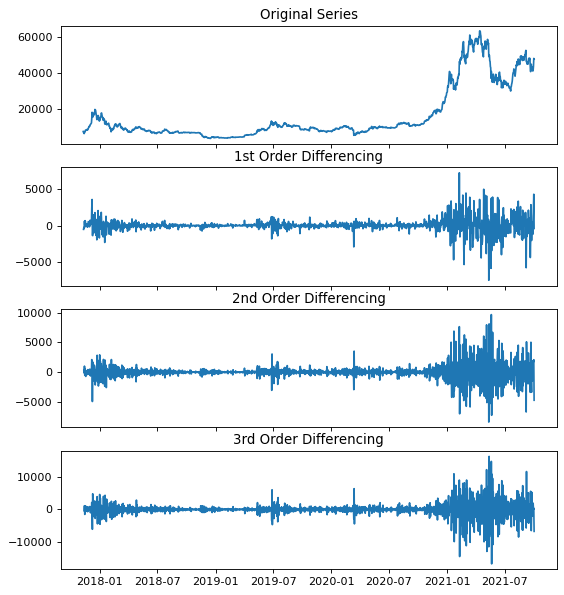
\includegraphics[width=0.495\textwidth]{./plots/arima/plots_btc/btc_1d_diff}}
  \subfloat[Autocorrelograma]{
   \label{f:fac}
    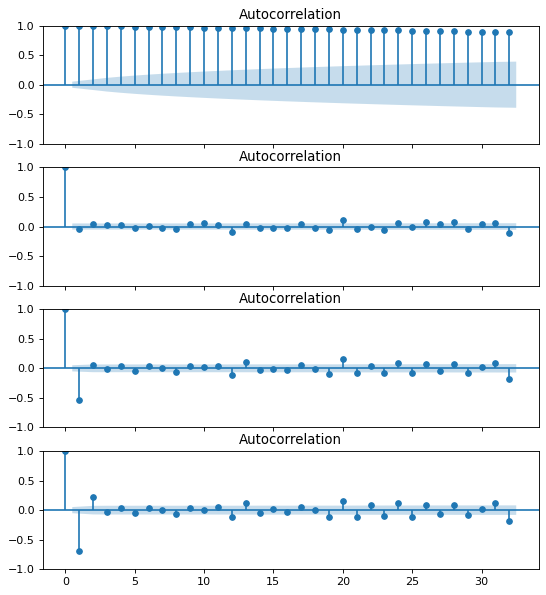
\includegraphics[width=0.48\textwidth]{./plots/arima/plots_btc/btc_1d_fac}}
  \caption{Sucesivas diferenciaciones y efecto en el autocorrelograma para la serie temporal de BTC con periodo de 1 día.}
  \label{f:btc_1d_diff-fac}
\end{figure}

\begin{figure}[h!]
 \centering
  \subfloat[$p=1$]{
   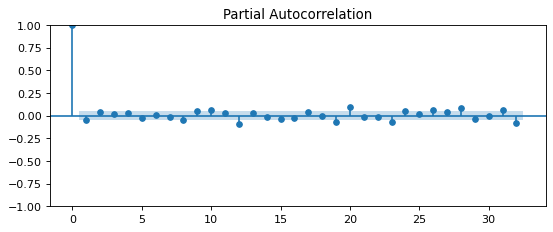
\includegraphics[width=0.5\textwidth]{./plots/arima/plots_btc/btc_1d_pac_p}}
  \subfloat[$p=2$]{
   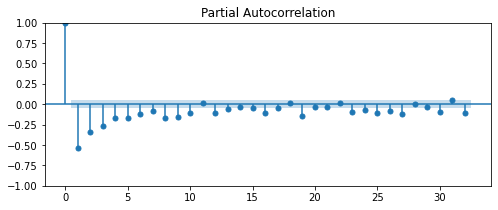
\includegraphics[width=0.5\textwidth]{./plots/arima/plots_btc/btc_1d_pac_p2}}
  \caption{Correlograma parcial de la diferenciación para el parámetro $p$}
  \label{f:fac_btc_p}
\end{figure}

\begin{figure}[h!]
 \centering
  \subfloat[$q=1$]{
   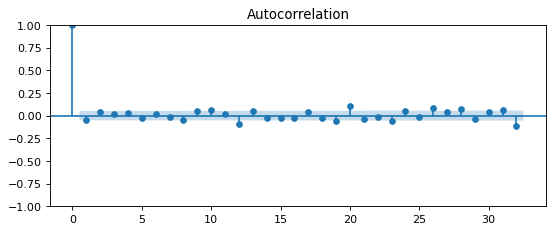
\includegraphics[width=0.5\textwidth]{./plots/arima/plots_btc/btc_1d_pac_q}}
  \subfloat[$q=2$]{
   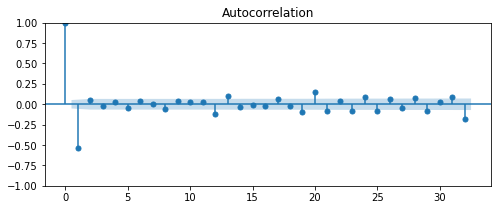
\includegraphics[width=0.5\textwidth]{./plots/arima/plots_btc/btc_1d_pac_q2}}
  \caption{Correlograma de la diferenciación para el parámetro $q$}
  \label{f:fac_btc_q}
\end{figure}

Con el fin de no extender y abrumar con gráficos y aún validar lo expuesto, para los restantes datasets se exhibirán los gráficos con los parámetros $p$ y $q$ elegidos, y la estacionariedad al variar $d$ en el Anexo I. En todos se encuentra un patrón común: $ARIMA(2,1,1)$

\subsubsection{Predicciones aleatorias}

Los gráficos (figura \ref{f:btc_wk_arima}) corresponden a el precio en un periodo de siete días del Bitcoin (tomados diez veces aleatoriamente), más otros siete días donde se compara la predicción del modelo y los valores reales. Las métricas pueden verse en el cuadro (\ref{tab:btc})

En tanto, la figura \ref{f:btc_mth_arima} recoge la misma información que los gráficos previamente presentados a excepción del modelo, que entrena con periodos de treinta días seleccionados aleatoriamente.

Los datasets utilizados fueron aquellos con periodos de un día.

Los entrenamientos correspondientes a las criptomonedas ADA y ETH se encuentran en el Anexo II.

\begin{figure}[h]
 \centering
  \subfloat[]{
   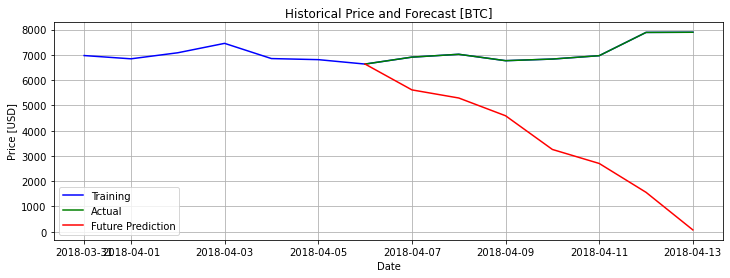
\includegraphics[width=0.5\textwidth]{./plots/arima/plots_btc_random_weekly/btc_wk1}}
  \subfloat[]{
   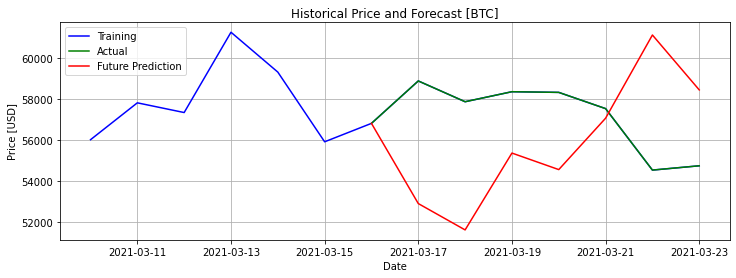
\includegraphics[width=0.5\textwidth]{./plots/arima/plots_btc_random_weekly/btc_wk2}} \\
  \subfloat[]{
   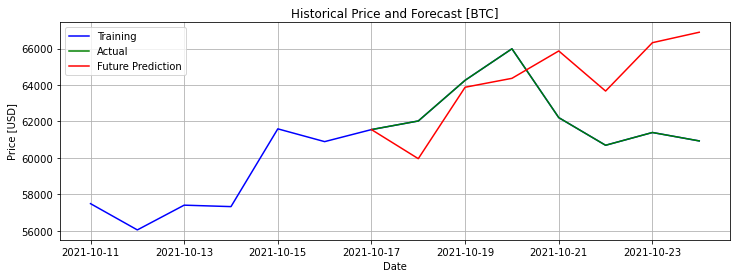
\includegraphics[width=0.5\textwidth]{./plots/arima/plots_btc_random_weekly/btc_wk3}}
   \subfloat[]{
   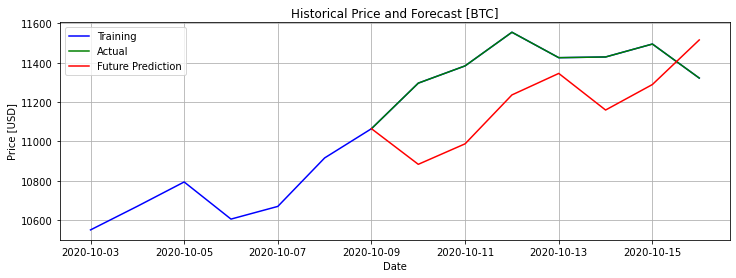
\includegraphics[width=0.5\textwidth]{./plots/arima/plots_btc_random_weekly/btc_wk4}} \\
   \subfloat[]{
   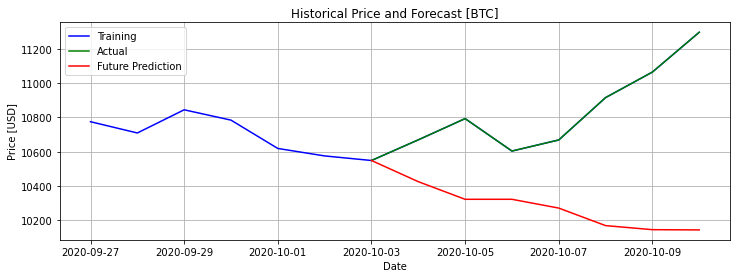
\includegraphics[width=0.5\textwidth]{./plots/arima/plots_btc_random_weekly/btc_wk5}}
   \subfloat[]{
   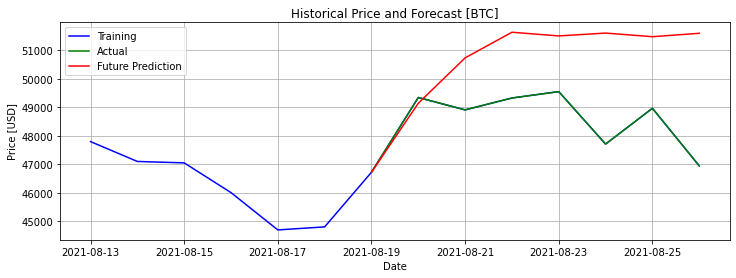
\includegraphics[width=0.5\textwidth]{./plots/arima/plots_btc_random_weekly/btc_wk6}} \\
   \subfloat[]{
   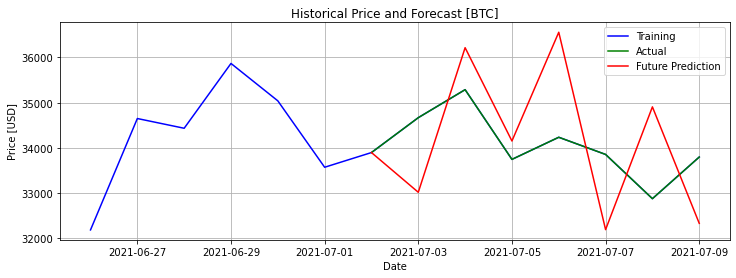
\includegraphics[width=0.5\textwidth]{./plots/arima/plots_btc_random_weekly/btc_wk7}}
   \subfloat[]{
   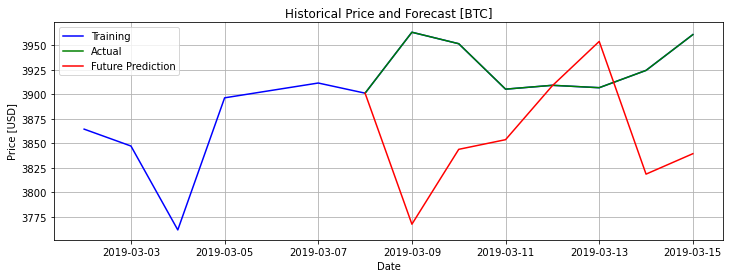
\includegraphics[width=0.5\textwidth]{./plots/arima/plots_btc_random_weekly/btc_wk8}} \\
   \subfloat[]{
   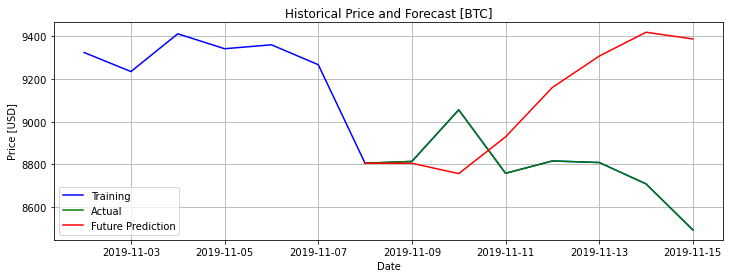
\includegraphics[width=0.5\textwidth]{./plots/arima/plots_btc_random_weekly/btc_wk9}}
   \subfloat[]{
   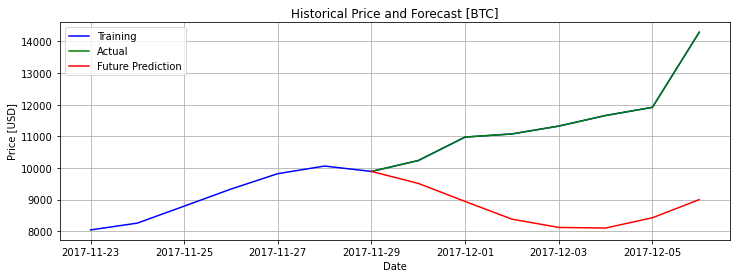
\includegraphics[width=0.5\textwidth]{./plots/arima/plots_btc_random_weekly/btc_wk10}}
  \caption{Predicción del modelo entrenado con 10 semanas aleatorias de BTC}
  \label{f:btc_wk_arima}
\end{figure}

\begin{table}[h]
 \begin{center}
  \begin{tabular}{|r|c|c|c|c|c|c|c|c|c|c|}
    Métrica & (a) & (b) & (c) & (d) & (e) & (f) & (g) & (h) & (i) & (j) \\ \hline
    MAE & 3886 & 4243 & 3088 & 268.4 & 600.9 & 2476 & 1495 & 90.04 & 418.8 & 3001 \\
    RMSE & 4499 & 4703 & 3573 & 290.1 & 680.4 & 2817 & 1611 & 107.5 & 506.8 & 3276 \\
    MAPE & 0.526 & 0.074 & 0.050 & 0.023 & 0.055 & 0.051 & 0.044 & 0.023 & 0.048 & 0.250 \\ \hline
  \end{tabular}
  \caption{Métricas de la figura \ref{f:btc_wk_arima}}
  \label{tab:btc}
 \end{center}
\end{table}

Para nuestro análisis, tomaremos los ejemplos más significativos: \ref{f:btc_wk_arima}(a), \ref{f:btc_wk_arima}(b) y \ref{f:btc_wk_arima}(d).

$MAE$ se define como el promedio de los errores absolutos para cada una de las observaciones. Implícitamente podemos intuir que un valor mayor para la métrica es consecuencia de un conjunto de predicciones bastante alejados de la realidad, o la presencia de puntos anómalos. La figura (b) muestra con claridad que la predicción no es nada buena. Del mismo modo, según el cuadro \ref{tab:btc}, le corresponde el valor más alto conferido por la métrica respecto a las demás observaciones. Por otro lado, la figura (d) contiene predicciones más cercanas (al menos, de forma relativa): buscando la métrica, vemos que corresponde a una de las más bajas.

¿Podemos concluir que valores más bajos de MAE sugieren una mejor predicción?

No. El problema de afirmar la pregunta es que ignora la evolución de los precios. Sin dudas obtendríamos la métrica increiblemente baja si tomamos algún periodo del 2017 en lugar de algún periodo de 2021. Particularmente, al obtener valores tan altos, sí podría señalarnos que la predicción no es la deseada.

La métrica MAPE es una medida porcentual\footnote{Los datos recopilados en el cuadro, sin embargo, no estan expresados porcentualmente.} cuyos valores más pequeños indican un mejor ajuste. El gráfico (a) acierta correctamente en esto, otorgando un $52.6\%$ de error a la predicción. En línea con lo anterior, observamos que para (b) otorga un 7.4\% -un valor, a simple vista, realmente malo- y para (d) un 2.3\%, quizás más aceptable subjetivamente.

\begin{figure}
 \centering
  \subfloat[]{
   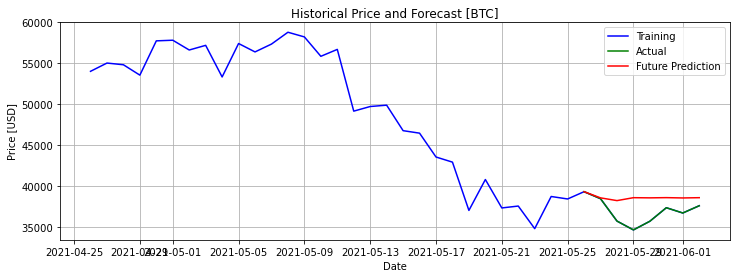
\includegraphics[width=0.5\textwidth]{./plots/arima/plots_btc_random_monthly/btc_mth1}}
  \subfloat[]{
   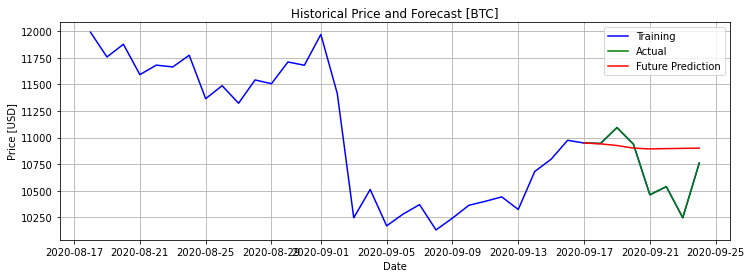
\includegraphics[width=0.5\textwidth]{./plots/arima/plots_btc_random_monthly/btc_mth2}} \\
  \subfloat[]{
   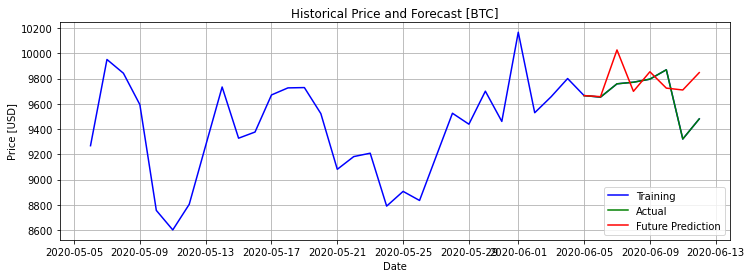
\includegraphics[width=0.5\textwidth]{./plots/arima/plots_btc_random_monthly/btc_mth3}}
   \subfloat[]{
   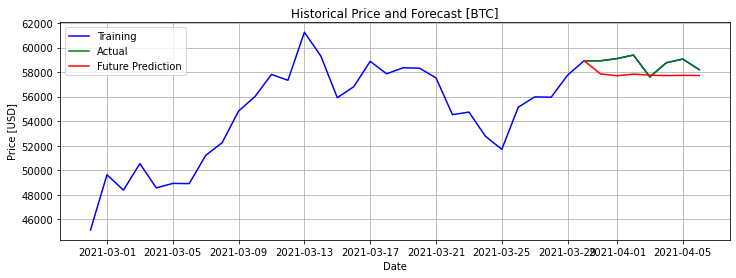
\includegraphics[width=0.5\textwidth]{./plots/arima/plots_btc_random_monthly/btc_mth4}} \\
   \subfloat[]{
   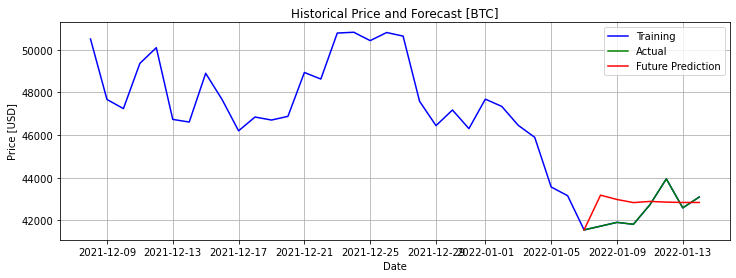
\includegraphics[width=0.5\textwidth]{./plots/arima/plots_btc_random_monthly/btc_mth5}}
   \subfloat[]{
   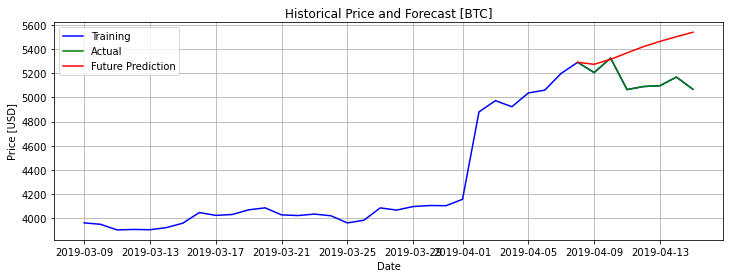
\includegraphics[width=0.5\textwidth]{./plots/arima/plots_btc_random_monthly/btc_mth6}} \\
   \subfloat[]{
   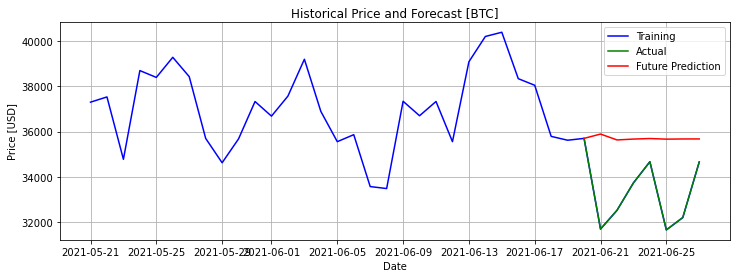
\includegraphics[width=0.5\textwidth]{./plots/arima/plots_btc_random_monthly/btc_mth7}}
   \subfloat[]{
   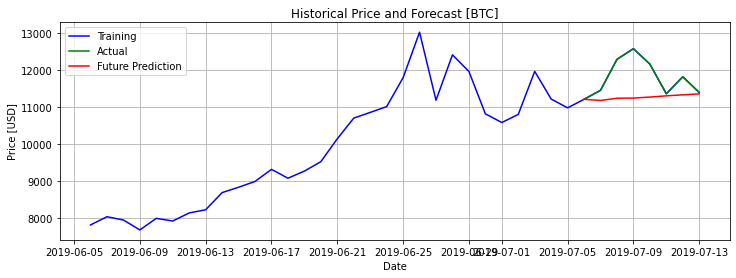
\includegraphics[width=0.5\textwidth]{./plots/arima/plots_btc_random_monthly/btc_mth8}} \\
   \subfloat[]{
   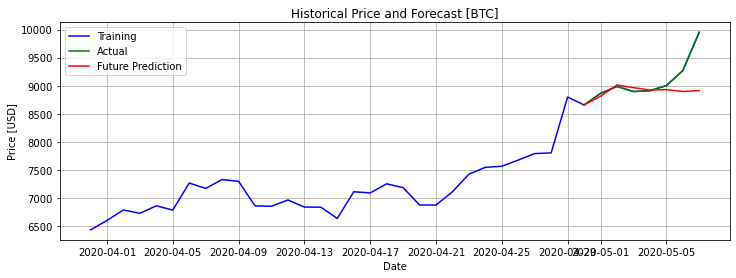
\includegraphics[width=0.5\textwidth]{./plots/arima/plots_btc_random_monthly/btc_mth9}}
   \subfloat[]{
   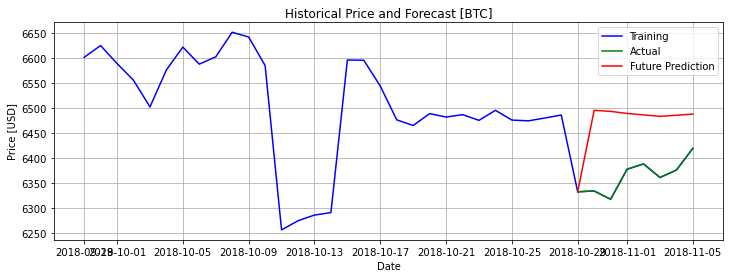
\includegraphics[width=0.5\textwidth]{./plots/arima/plots_btc_random_monthly/btc_mth10}}
  \caption{Predicción del modelo entrenado con 10 meses aleatorios de BTC}
  \label{f:btc_mth_arima}
\end{figure}

\begin{table}[t]
 \begin{center}
  \begin{tabular}{|r|c|c|c|c|c|c|c|c|c|c|}
    Métrica & (a) & (b) & (c) & (d) & (e) & (f) & (g) & (h) & (i) & (j) \\ \hline
    MAE & 1924 & 255.9 & 186.1 & 1003 & 756.4 & 268.8 & 2692 & 588.8 & 233.9 & 121.2 \\
    RMSE & 2264 & 335.8 & 235.0 & 1111 & 897.0 & 309.9 & 2970 & 753.8 & 418.3 & 125.9 \\
    MAPE & 0.054 & 0.024 & 0.019 & 0.017 & 0.017 & 0.053 & 0.083 & 0.048 & 0.024 & 0.019 \\ \hline
  \end{tabular}
  \caption{Métricas de la figura \ref{f:btc_mth_arima}}
  \label{tab:btc_wk}
 \end{center}
\end{table}







\subsection{Prophet}

\subsubsection{Predicciones Aleatorias}

Los ajustes fueron generados automáticamente por Prophet, incluyendo los puntos de cambio de tendencia. Vemos que, si bien este ajuste no fue malo, puede mejorar o aproximarse más a los resultados reales si determinamos una mayor flexibilidad en estos puntos de corte.

Hay mucha incertidumbre en los modelos con poco entrenamiento. Esto se vé reflejado en las métricas publicadas, las cuales mejoraron al ampliar el conjunto de entrenamiento.

Esta biblioteca funciona muy bien siempre y cuando los datos no presenten alta frecuencia ni horizontes de predicción muy cortos, ya que los datos pueden no ser suficientes para
determinar la estacionalidad o pueden variar mucho como para establecer la periodicidad (ver figura \ref{f:btc_mth_prophet}(f) respecto a (h)).

\begin{figure}[h!]
 \centering
  \subfloat[]{
   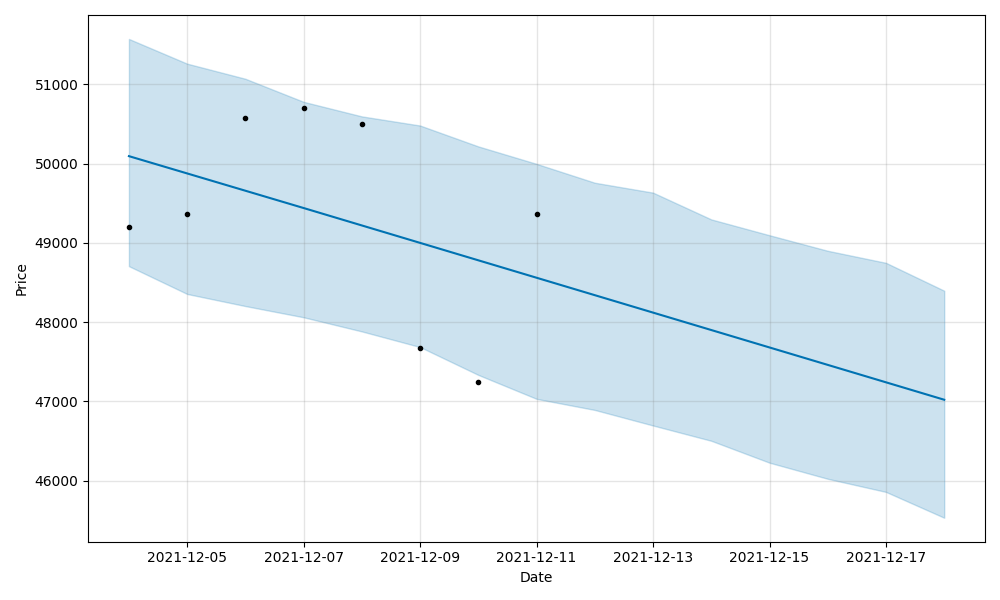
\includegraphics[width=0.45\textwidth]{./plots/prophet/btc/week/1}}
  \subfloat[]{
   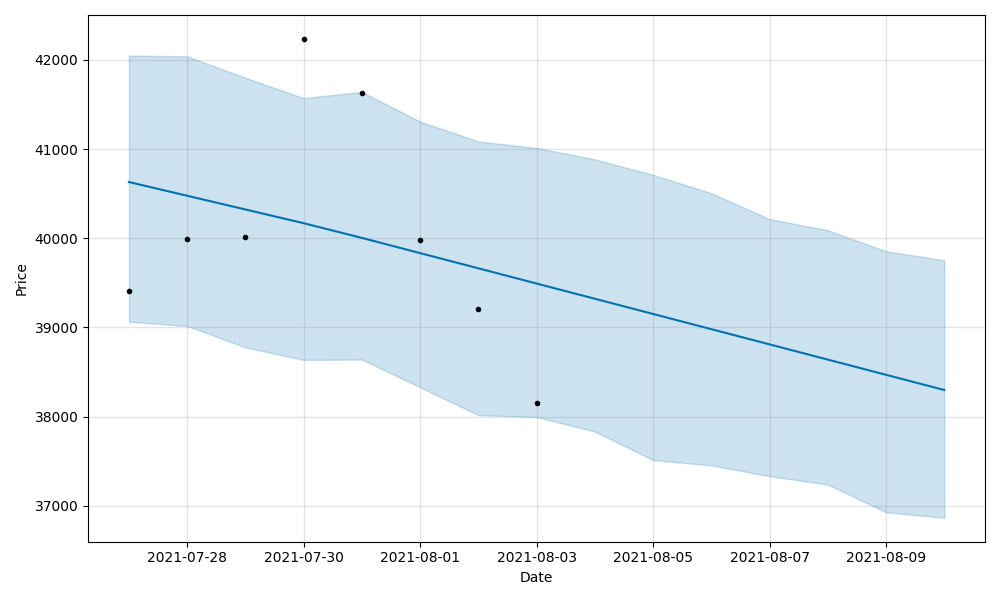
\includegraphics[width=0.45\textwidth]{./plots/prophet/btc/week/2}} \\
  \subfloat[]{
   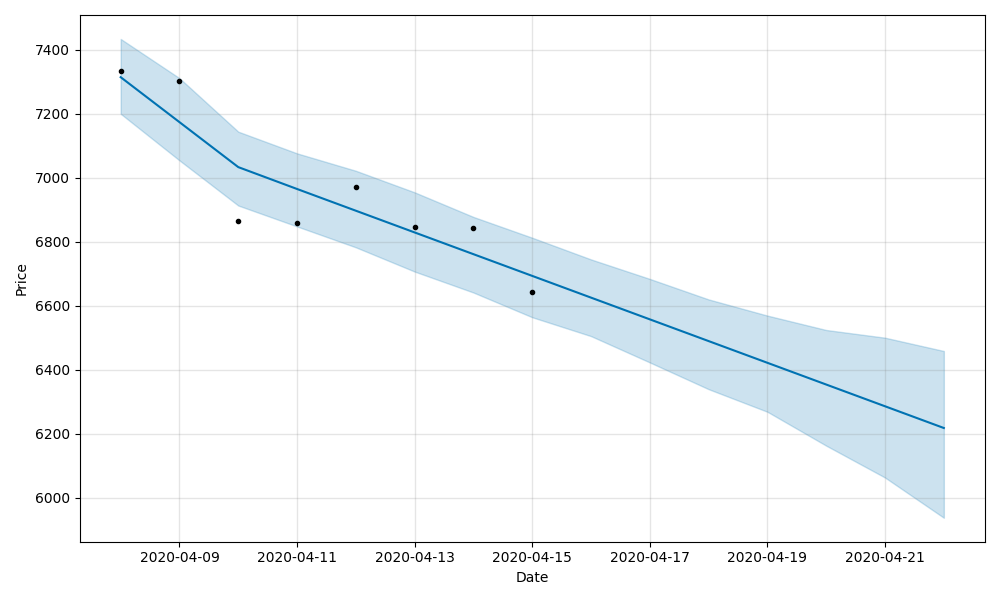
\includegraphics[width=0.45\textwidth]{./plots/prophet/btc/week/3}}
   \subfloat[]{
   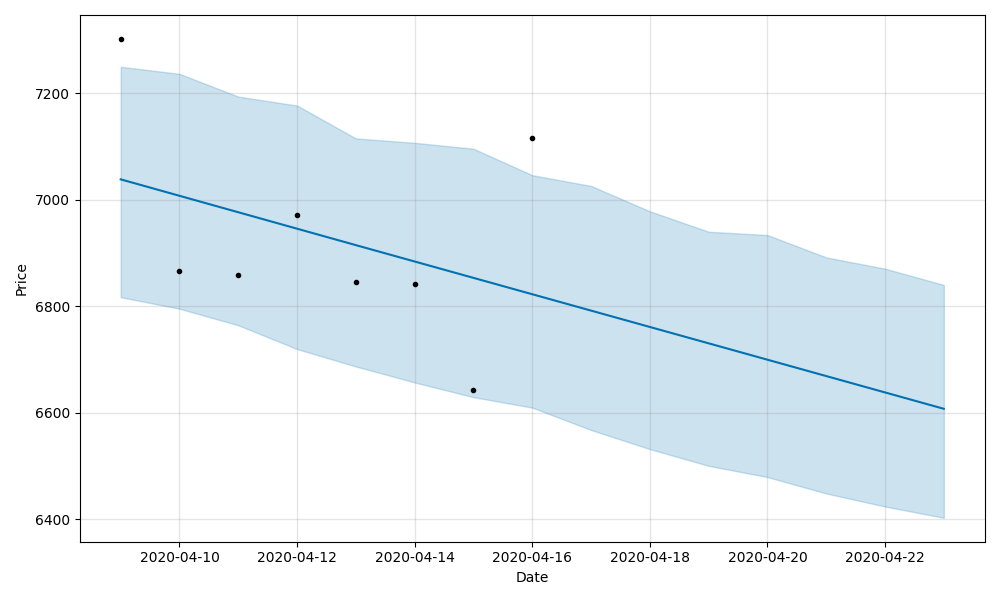
\includegraphics[width=0.45\textwidth]{./plots/prophet/btc/week/4}} \\
   \subfloat[]{
   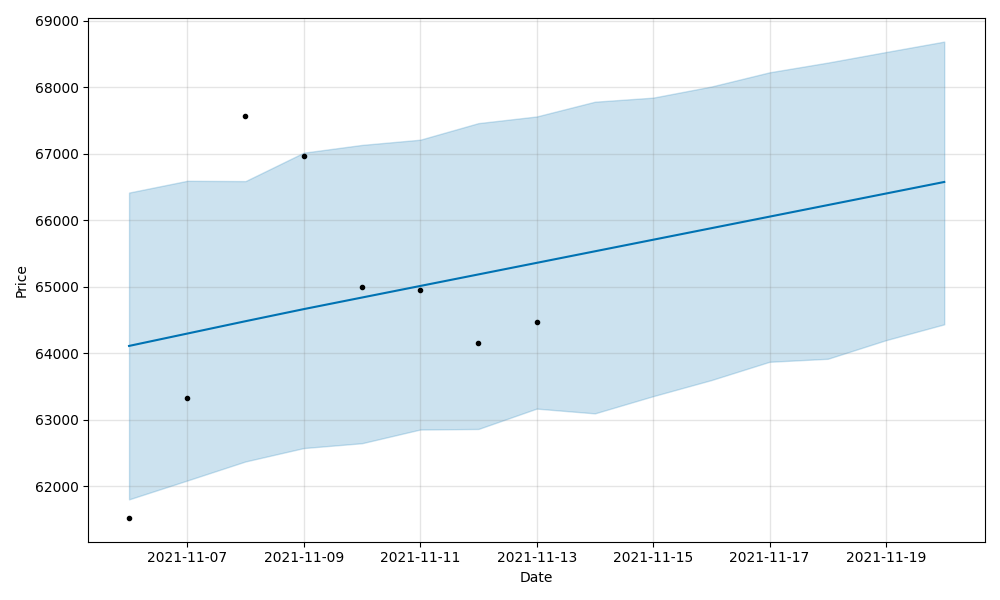
\includegraphics[width=0.45\textwidth]{./plots/prophet/btc/week/5}}
   \subfloat[]{
   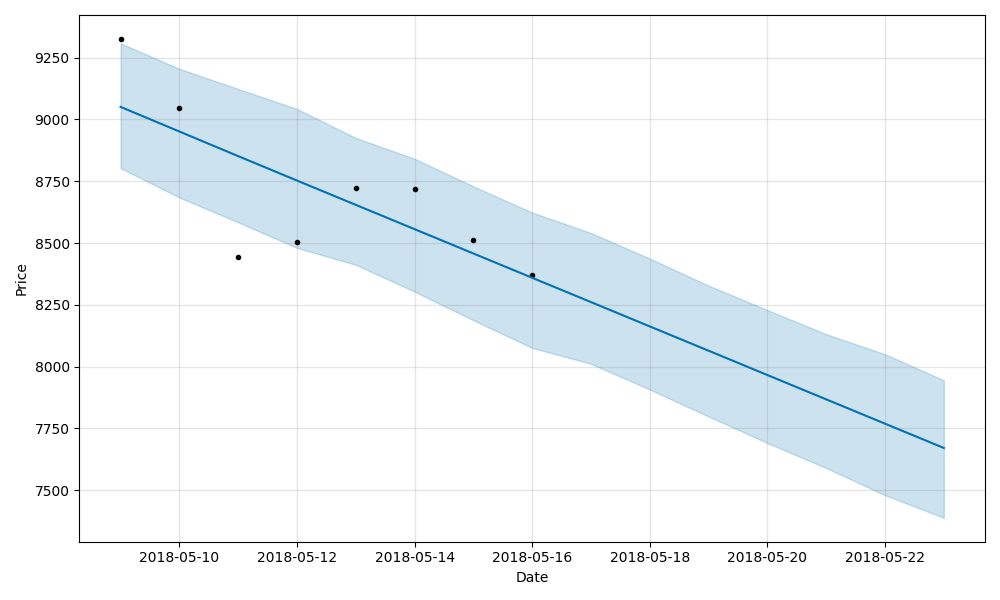
\includegraphics[width=0.45\textwidth]{./plots/prophet/btc/week/6}} \\
   \subfloat[]{
   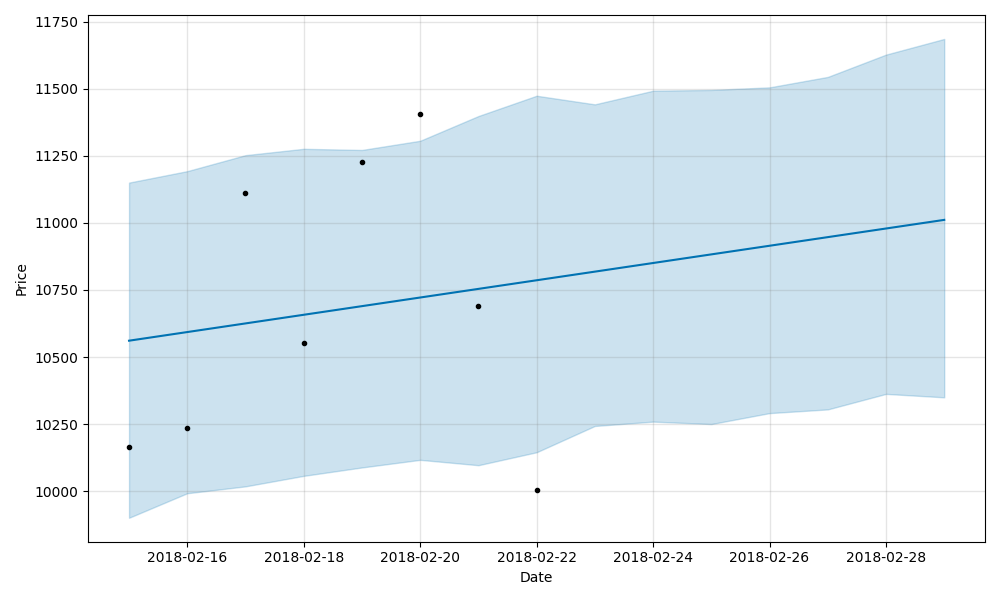
\includegraphics[width=0.45\textwidth]{./plots/prophet/btc/week/7}}
   \subfloat[]{
   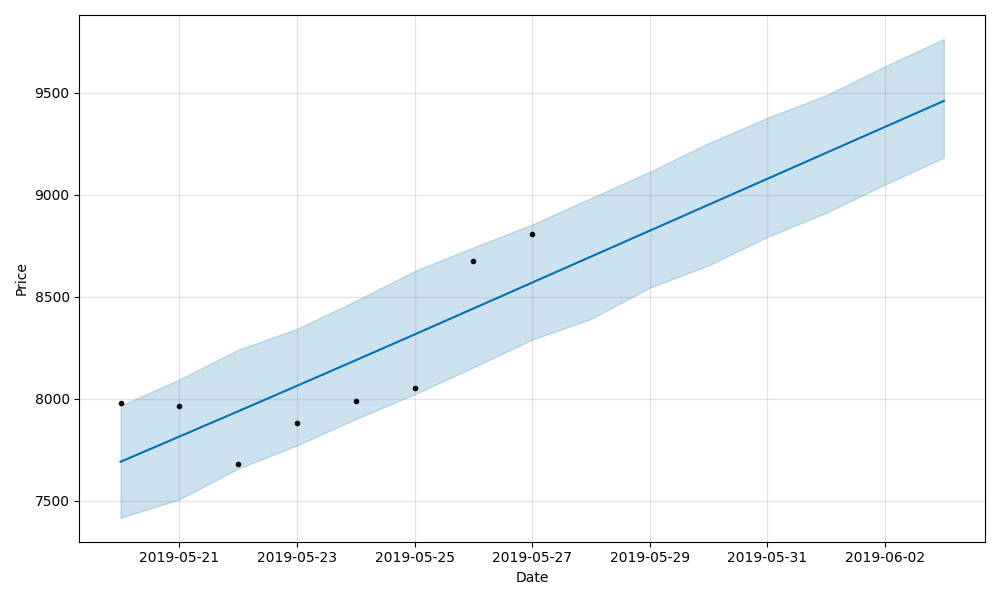
\includegraphics[width=0.45\textwidth]{./plots/prophet/btc/week/8}} \\
   \subfloat[]{
   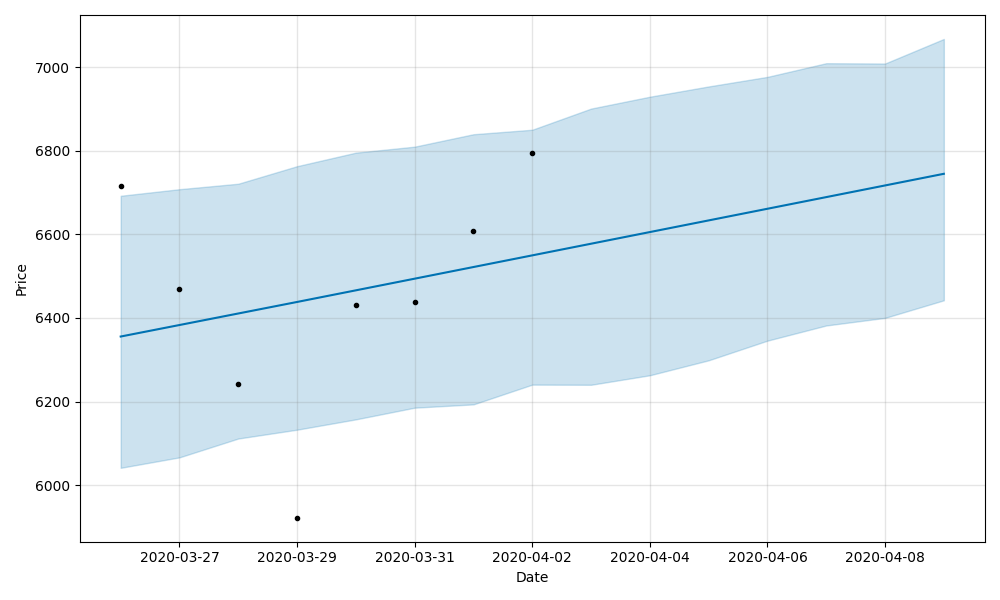
\includegraphics[width=0.45\textwidth]{./plots/prophet/btc/week/9}}
   \subfloat[]{
   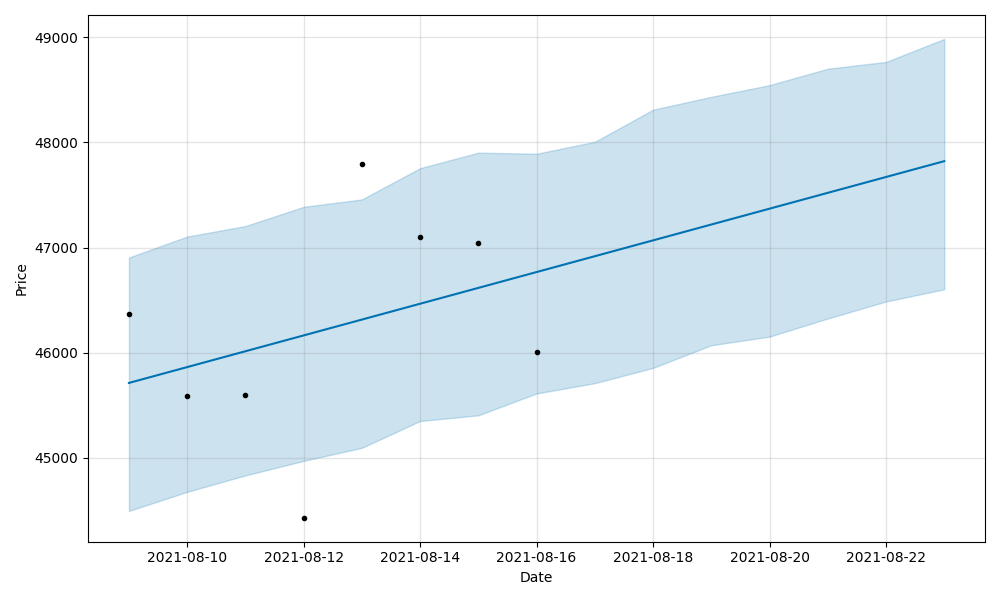
\includegraphics[width=0.45\textwidth]{./plots/prophet/btc/week/10}}
  \caption{Predicción del modelo entrenado con 10 semanas aleatorias de BTC}
  \label{f:btc_wk_prophet}
\end{figure}

\begin{table}[h!]
 \begin{center}
  \begin{tabular}{|r|c|c|c|c|c|c|c|c|c|c|}
    Métrica & (a) & (b) & (c) & (d) & (e) & (f) & (g) & (h) & (i) & (j) \\ \hline
    MAE & 65.19 & 1616 & 2386 & 25018 & 9654 & 14195 & 633.9 & 78.68 & 1803 & 3678 \\
    RMSE & 65.19 & 1616 & 2386 & 25018 & 9654 & 14195 & 633.9 & 78.68 & 1803 & 3678 \\
    MAPE & 0.017 & 0.032 & 0.293 & 0.402 & 0.149 & 0.379 & 0.063 & 0.012 & 0.265 & 0.087 \\ \hline
  \end{tabular}
  \caption{Métricas de la figura \ref{f:btc_wk_prophet}}
  \label{tab:btc_prophet_wk}
 \end{center}
\end{table}

\begin{figure}[h!]
 \centering
  \subfloat[]{
   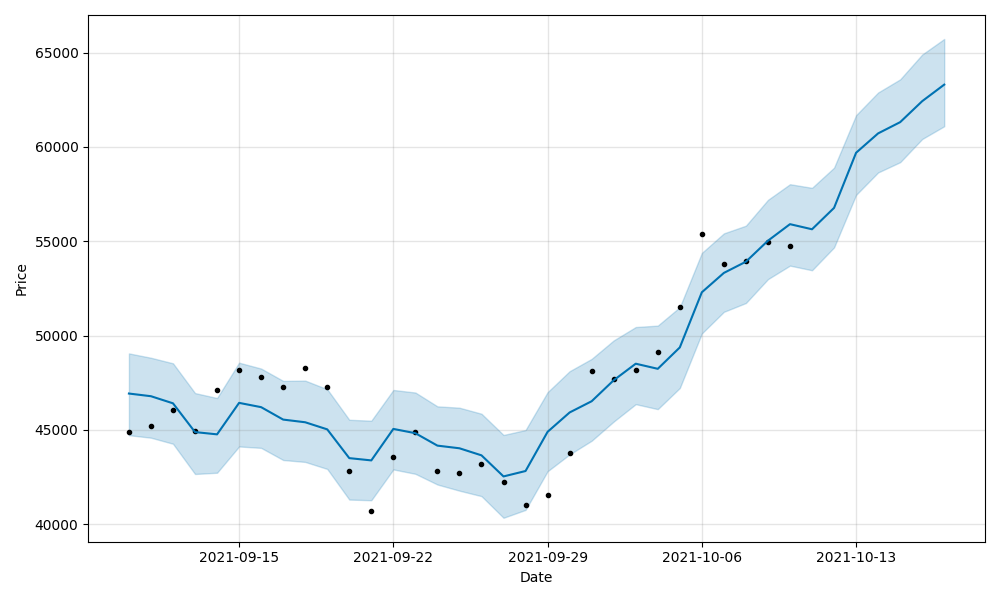
\includegraphics[width=0.45\textwidth]{./plots/prophet/btc/month/1}}
  \subfloat[]{
   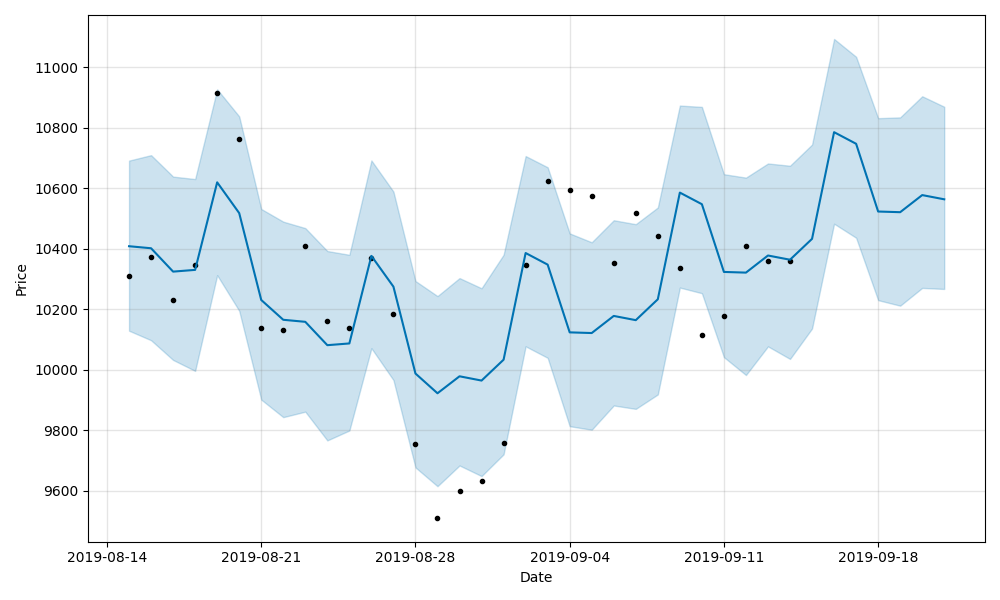
\includegraphics[width=0.45\textwidth]{./plots/prophet/btc/month/2}} \\
  \subfloat[]{
   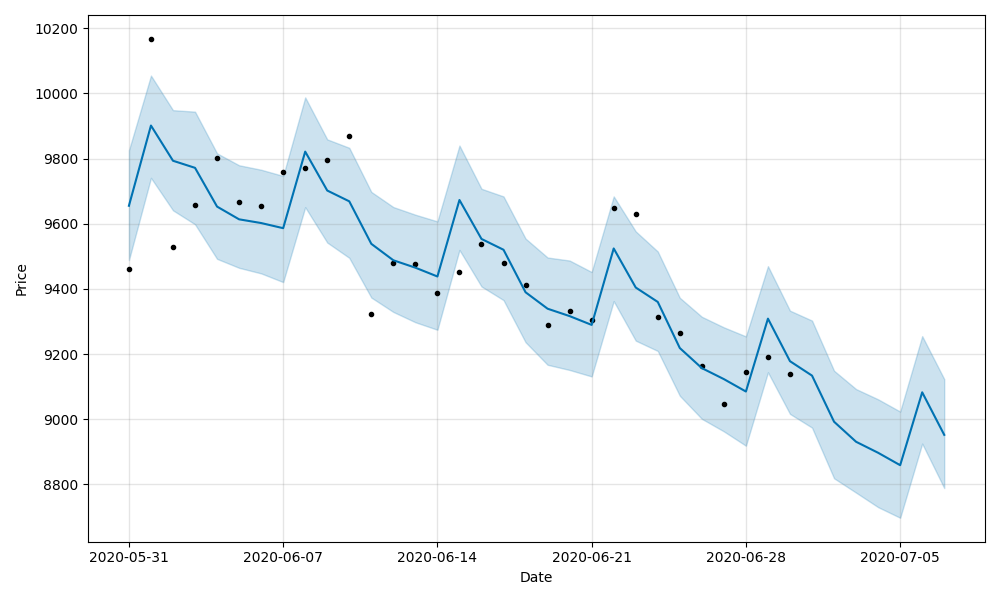
\includegraphics[width=0.45\textwidth]{./plots/prophet/btc/month/3}}
   \subfloat[]{
   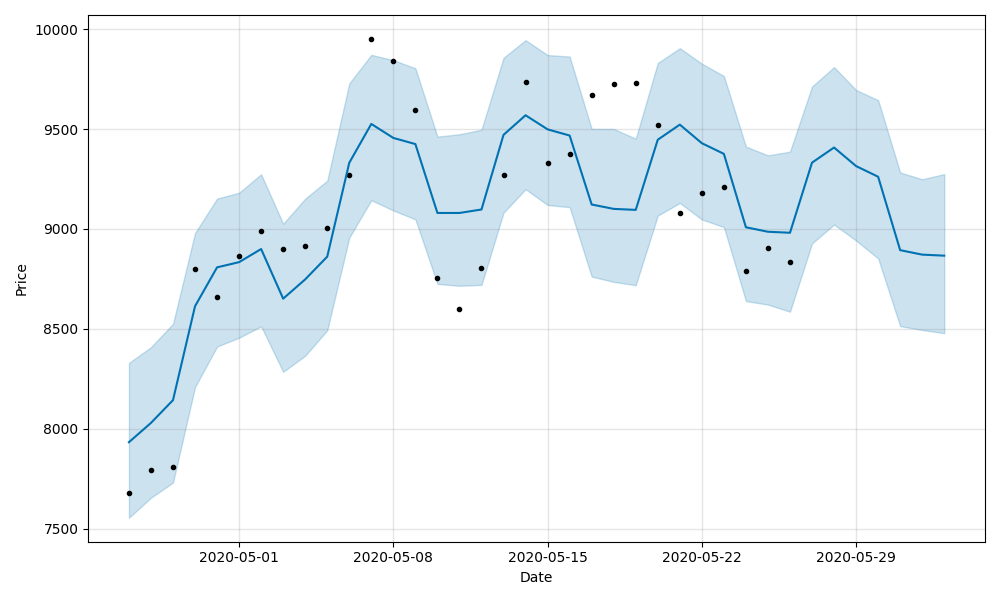
\includegraphics[width=0.45\textwidth]{./plots/prophet/btc/month/4}} \\
   \subfloat[]{
   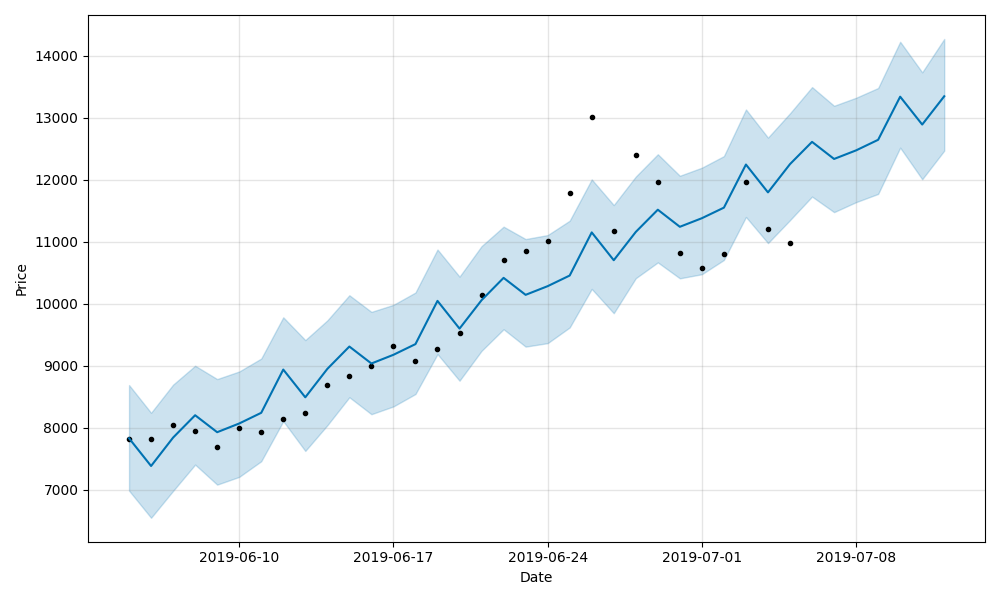
\includegraphics[width=0.45\textwidth]{./plots/prophet/btc/month/5}}
   \subfloat[]{
   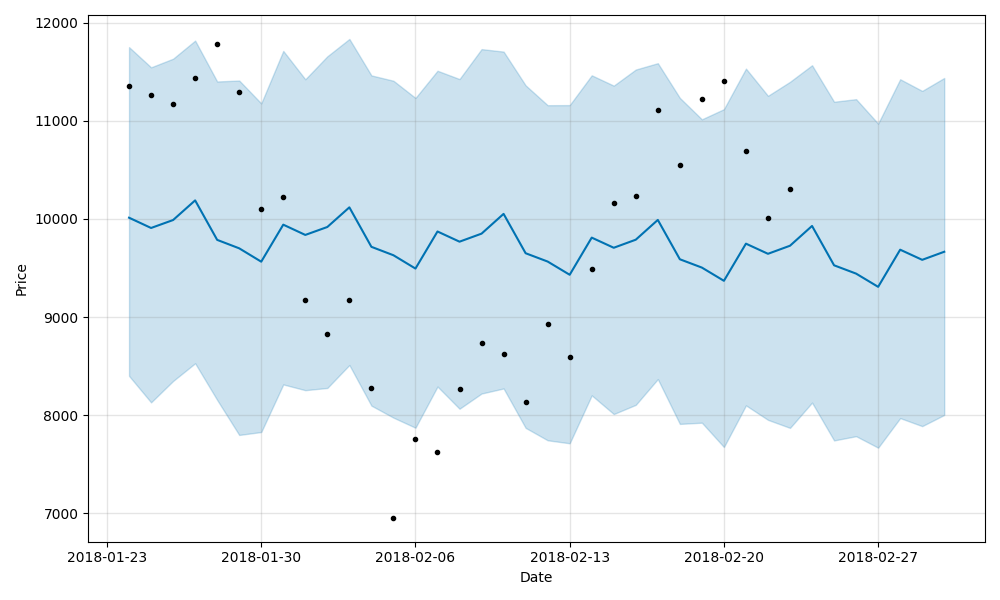
\includegraphics[width=0.45\textwidth]{./plots/prophet/btc/month/6}} \\
   \subfloat[]{
   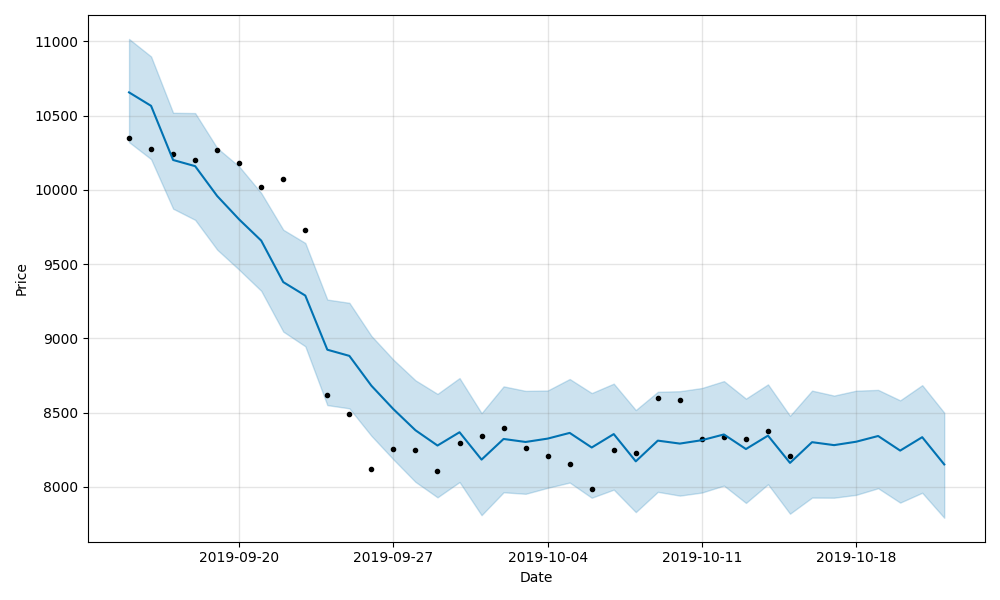
\includegraphics[width=0.45\textwidth]{./plots/prophet/btc/month/7}}
   \subfloat[]{
   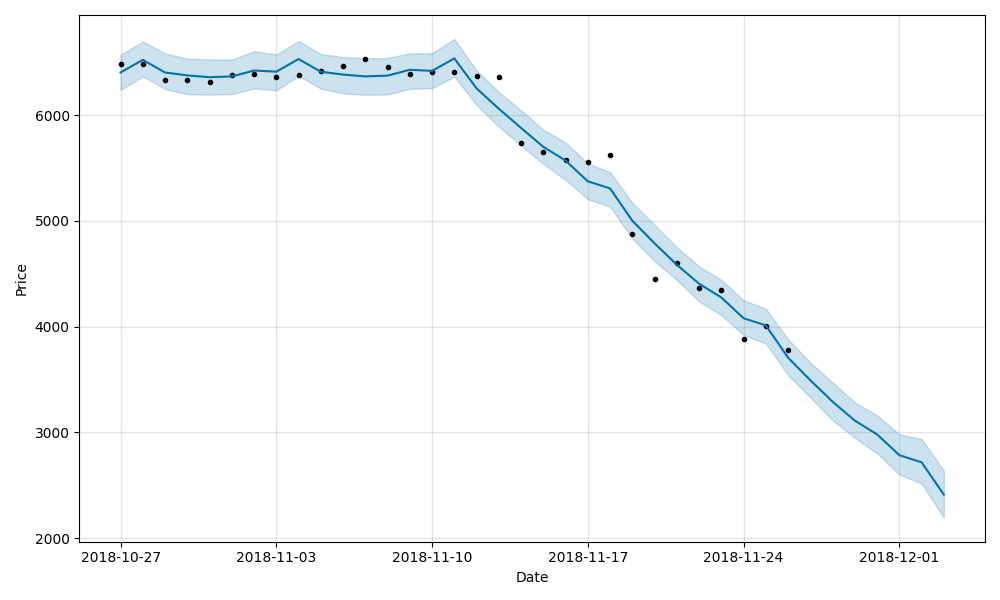
\includegraphics[width=0.45\textwidth]{./plots/prophet/btc/month/8}} \\
   \subfloat[]{
   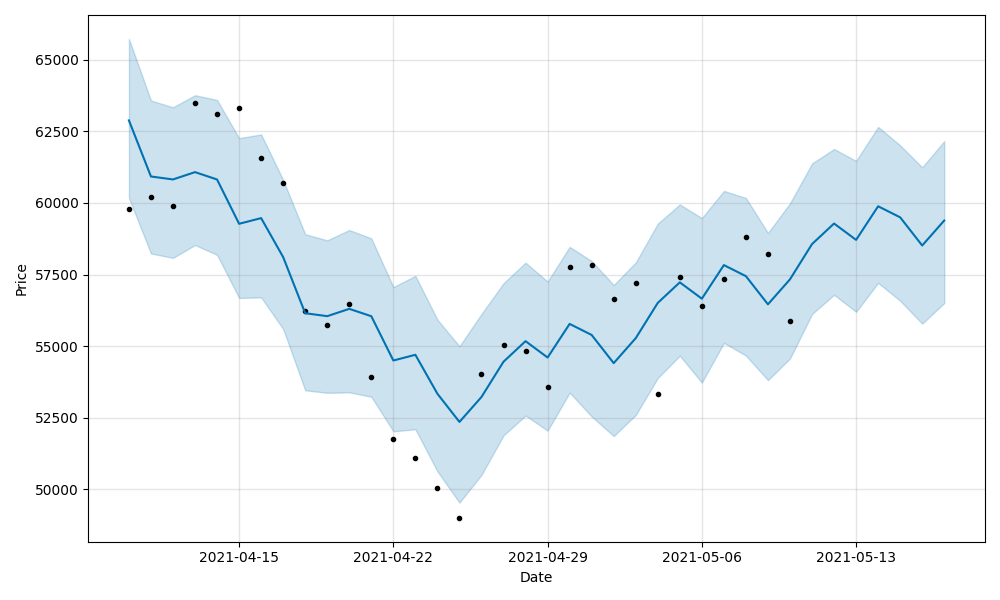
\includegraphics[width=0.45\textwidth]{./plots/prophet/btc/month/9}}
   \subfloat[]{
   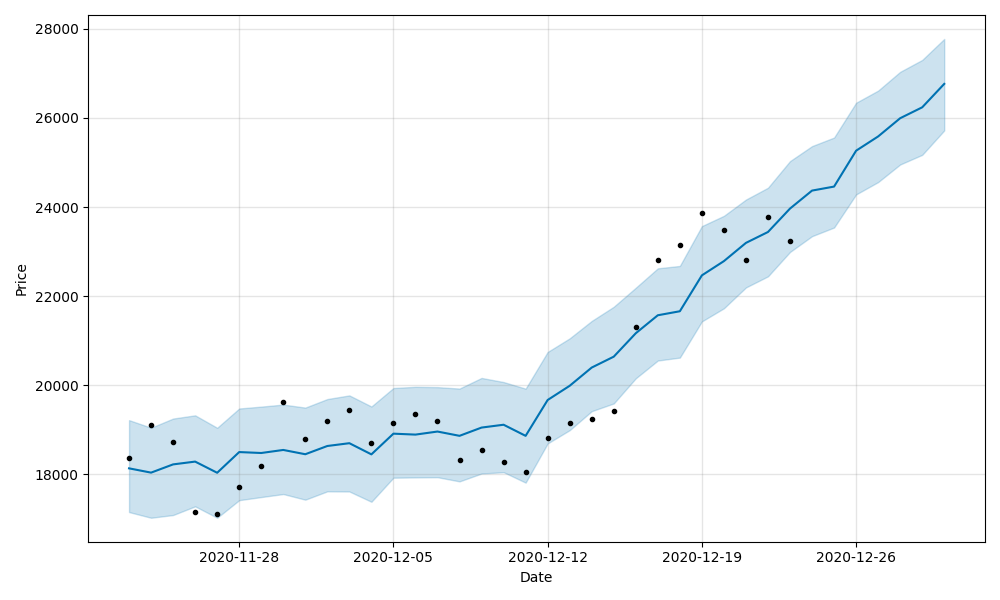
\includegraphics[width=0.45\textwidth]{./plots/prophet/btc/month/10}}
  \caption{Predicción del modelo entrenado con 10 meses aleatorios de BTC}
  \label{f:btc_mth_prophet}
\end{figure}

\begin{table}[t]
 \begin{center}
  \begin{tabular}{|r|c|c|c|c|c|c|c|c|c|c|}
    Métrica & (a) & (b) & (c) & (d) & (e) & (f) & (g) & (h) & (i) & (j) \\ \hline
    MAE & 62931 & 20152 & 196094 & 19753 & 34188 & 11018 & 246692 & 21603 & 62265 & 26942 \\
    RMSE & 87618 & 27940 & 274664 & 27251 & 45858 & 15213 & 174472 & 30480 & 85150 & 36169 \\
    MAPE & 7.543 & 3.136 & 4.508 & 2.217 & 4.099 & 1.590 & 18.68 & 5.589 & 1.108 & 1.49 \\ \hline
  \end{tabular}
  \caption{Métricas de la figura \ref{f:btc_mth_prophet}}
  \label{tab:btc_prophet_m}
 \end{center}
\end{table}




\subsection{Comparación de Modelos}

Como se adelantó previamente, para esta comparativa se eligió cuatro periodos de treinta días de entrenamiento para cada modelo. Los pronósticos son a siete días y se pueden observar en la figura \ref{f:btc_ax_ph}.

Las métricas obtenidas (figuras \ref{f:corr}, \ref{f:mae}, \ref{f:mape}) son las utilizadas con anterioridad pero esta vez junto al coeficiente de correlación (ver 1.2.2). Este coeficiente es una medida de dependencia lineal entre dos variables aleatorias\footnote{\url{https://es.wikipedia.org/wiki/Coeficiente_de_correlacion_de_Pearson}}. Un valor $0<|r|<1$ indica una fuerza mayor entre las variables involucradas. El signo de $r$ es significativo en otros contextos a excepción del presente, por lo cual se ignora con el fin de presentar el gráfico de barras.

Como puede apreciarse en la figura, se calcula la correlación para los pares ARIMA-Actual (valores reales), Prophet-Actual y ARIMA-Prophet. Este último con el fin de determinar la diferencia (o igualdad) de sus pronósticos.

\begin{itemize}

 \item La correlación (figura \ref{f:corr}(a)) para la predicción \ref{f:btc_ax_ph}(a) nos da valores relativamente altos e iguales. Entre ellos, Prophet es el más acertado en la cercanía de curvas. Sin embargo, el coeficiente es cercano al de ARIMA, cuyo desempeño es malo.

 Para las restantes predicciones, ARIMA no brinda información relevante (\ref{f:btc_ax_ph}(b), (c), (d)) variando el coeficiente en valores muy bajos, medios y relativamente altos (\ref{f:corr}(b), (d) y (c) respectivamente). Prophet, en cambio, logra un desempeño más aceptable, capturando dos tendencias (\ref{f:btc_ax_ph}(c) y (d)) con un coeficiente mayor a 0.5 y una negativa total en (b) cuyo coeficiente es muy cercano a 0.

 \begin{figure}[h!]
 \centering
  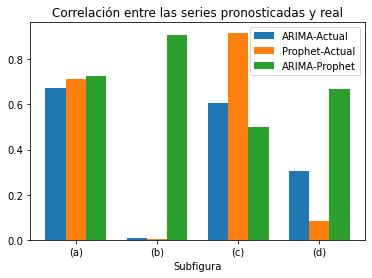
\includegraphics[width=0.7\textwidth]{./plots/btc_ax_ph/corr}
  \caption{Coeficiente de correlación para las predicciones de la figura \ref{f:btc_ax_ph}}
  \label{f:corr}
\end{figure}

 \item La métrica MAE, en Prophet, acierta considerablemente respecto a \ref{f:btc_ax_ph}(a), (b) y (d), con valores altos y bajos, aunque (d) es cuestionable al existir diferencias contrarrestadas entre los primeros tres días y los cuatro restantes. Un caso interesante es la cercanía de curvas en (c): a pesar del poco error entre cada punto, la media entre ellos tiende a crecer por la tendencia de la serie.

 La métrica para el modelo ARIMA es consistente únicamente en \ref{f:btc_ax_ph}(b). Apreciése (d); es esperable un MAE más alto (alrededor de 3000) pero la presencia de una predicción muy cercana altera totalmente el resultado.

 \begin{figure}[h!]
 \centering
   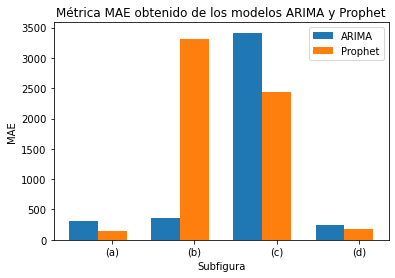
\includegraphics[width=0.7\textwidth]{./plots/btc_ax_ph/mae}
  \caption{Métrica MAE para las predicciones de la figura \ref{f:btc_ax_ph}}
  \label{f:mae}
\end{figure}

 \item MAPE, recordando que se entiende de una medida de error de pronóstico, no es acertado en ARIMA: \ref{f:btc_ax_ph}(b) indicaría que existe un 2\%, en promedio, de error de pronóstico pero para \ref{f:btc_ax_ph}(d) un 6\% (algo no plasmado en el gráfico, irónicamente).

 En Prophet se observa resultados más aceptables; incluso el mayor valor \ref{f:mape}(d) corresponde con errores mayores. Particularmente, \ref{f:mape}(b) no exhibe lo que muestra \ref{f:btc_ax_ph}(b) explicable por los valores reales muy por encima de los predecidos.


 \begin{figure}[h!]
 \centering
   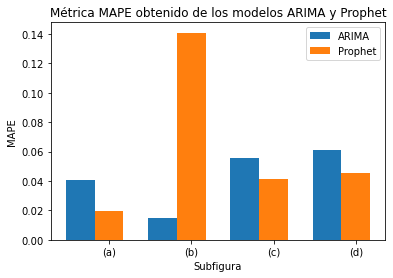
\includegraphics[width=0.7\textwidth]{./plots/btc_ax_ph/mape}
  \caption{Métrica MAPE para las predicciones de la figura \ref{f:btc_ax_ph}}
  \label{f:mape}
\end{figure}

\end{itemize}



\begin{figure}[h!]
 \centering
  \subfloat[]{
   \includegraphics[width=0.5\textwidth]{./plots/btc_ax_ph/1}}
  \subfloat[]{
   \includegraphics[width=0.5\textwidth]{./plots/btc_ax_ph/2}} \\
  \subfloat[]{
   \includegraphics[width=0.5\textwidth]{./plots/btc_ax_ph/3}}
   \subfloat[]{
   \includegraphics[width=0.5\textwidth]{./plots/btc_ax_ph/4}} \\
  \caption{Cuatro predicciones del BTC de ambos modelos}
  \label{f:btc_ax_ph}
\end{figure}







\section{Conclusión}

Los dos modelos estudiados se rigen bajo un principio que las series temporales de las criptomonedas analizadas no cumplen: la estacionalidad. Si bien mediante técnicas se busca que estas series alcancen la misma, en la práctica se observa que tienen limitaciones altísimas, aunque con alguna excepción digna por parte del modelo generado por Prophet capturando tendencias pero generando el sentimiento contrario al encontrarse con comportamientos de alza o bajada extremos, como frecuentemente sucede en este tipo de mercados.

Las métricas, por su parte, han respondido en ocasiones muy bien -hablando exclusivamente de Prophet- aunque existen predicciones donde el ajuste de la curva no respondía numéricamente a ninguna de las métricas utilizadas. Es menester validar de forma más extensa el objetivo de este informe partiendo de modelos más complejos que ARIMA, tal como lo es Prophet, con la certeza de tener métricas que acompañan el proceso.





\end{document}
